%\documentclass[letter]{article}
\documentclass[letter,12pt]{article}
\usepackage[letterpaper,right=1.25in,left=1.25in,top=1in,bottom=1in]{geometry}
\usepackage{setspace}

\usepackage{hyperref}
\usepackage{url}
\usepackage[pdftex]{graphicx}
\usepackage[longnamesfirst, sort]{natbib}\bibpunct[]{(}{)}{,}{a}{}{;}
\usepackage{arydshln}
\usepackage{amsmath}

%\usepackage{rotating}
%\usepackage{pdflscape}

\newcommand{\mc}{\multicolumn}

\graphicspath{{../graphs/}}

\begin{document}

\title{Malapportionment, party bias, and responsiveness in Mexico's mixed-member system\thanks{We are grateful to Jonathan Slapin and participants of the Analyzing Latin American Politics conference, University of Houston, Nov.~14--15, 2014 for comments and critiques; and to IFE's Cartography Department for sharing their experience with automated redistricting since 1996 and most of the data we analyze. We also acknowledge the support from the Asociaci\'on Mexicana de Cultura A.C.\ and CONACYT for this work.}}
\author{Eric Magar \\ {\footnotesize \url{emagar@itam.mx}} \and
        Micah Altman \\ {\footnotesize \url{escience@mit.edu}} \and
        Michael P.~McDonald \\ {\footnotesize \url{michael.mcdonald@ufl.edu}} \and  %\\ University of Florida, Gainesville\\
        Alejandro Trelles \\ {\footnotesize \url{lat44@pitt.edu}}
      }
\date{\today}
\maketitle

\begin{abstract}
\noindent Automated redistricting in consultation with parties since 1997 rid redistricting in Mexico of the most flagrant distorsions on representation. But more subtle ones remain. Rules and practice introduce some degree of malapportionment, small in comparative perspective \citep{samuels.snyder.2001}, but nonetheless substantial. We inspect district maps, votes, and seats in Mexico in search for two forms of political distorsion that may arise from malapportionment: party bias and responsiveness (otherwise known as plurality bias). State-level data reveal no evidence of systematic party bias. What bias there is is of another kind, a big bonus for larger parties (or vote responsiveness) typical of plurality rule in single-member districts. Since most states distribute few seats each, the large party bonus of states' federal districts doubles the estimate with national data. Since the PRI is the largest party in most states, it receives a substantial seat bonus.
\end{abstract}

% Search James Parker Smith and the Royal Commission on Systems of Election 1909 for cube law's origins
% Working hypothesis should be that PRI gains from malapp. 
% Then an explanation of why we can't find it, despite substantial malapportionment: very large inter-election swings. 
% Slapin: Is is normatively bad to sacrifice 1 citizen 1 vote, or ok if that sacrifice done for other goals such as indigenous representation or municipal boundaries?
%
% Micah: use total votes instead of total population to measure malapportionment. Should capture which bastions exist, if they are packed, turnout differences (if measured against p18). 
% Mike: consejos distritales and staff are patronnage posts coveted by parties and bureaucrats, how does redistricting affect calculus. Blends well with the story of consejeros distritales as homeowners in cabecera that they wish not to change. 
% Other paper: touch issue of weights, units and components of cost function in general---rabbit burgers from how to lie with statistics, one unit of rabbit and one unit of cow... Eric: that humans beat the machine is proof that the algorithm stops at local minima quite easily. 

% Comment [Eric] The following looks promising
% comment [Mike] Bernie Grofman wrote a co-authored paper (I'll have to dig up the cite) that decomposed bias into apportionment, malapportionment, and redistricting effects. Perhaps we take a similar approach in future revisions? If the manuscript goes that direction, the apportionment section should go before redistricting since apportionment occurs before redistricting. 

% Comment [Eric] Dropped this, may be useful for framing of for discussion
% \begin{tabular}{l|c|c|}
%                   & \mc{2}{c}{Would 2013 have reverted?}\\ \cline{2-3}
% State is          & yes                  & no \\ \hline
% over-represented  & df oax pue sin       & bcs col\\ \hline
% under-represented &  cps gua que qui tam & ags bc cam coa dgo\\ \hline
%                   &                      & cua gue hgo mic mor  \\ 
% on target         & jal mex ver          & nay nl san son tab  \\ 
%                   &                      & tla yuc zac \\ \hline
% \end{tabular}



\onehalfspacing

% NEW INTRO
% In electoral systems partitioning the territory into districts for the purpose of seat allocation---as most, in fact, do \citep{taagepera.shugart.1989}(Taag Shug, Lij)---malapportionment occurs when sparsely populated areas get the same representation as the densely populated. It is a distorsion that invalidates the `one person, one vote' principle of representative democracy. Scholars have investigated the phenomenon and its consequences in the U.S. and the U.K. well---where reformers succeeded in mostly removing it (Ansol et al, Cox Katz, Johns)---but remains understudied elsewhere (Jack, Sam Sny)

% Mexico's countryside has been losing relative population in favor of urban areas for decades. We show that demographic shifts in conjunction with legal lags, are responsible for substantial malapportionment in Mex. 

% It also has a apopulation largely matching the PRI's traditional bases of electoral support: rural population, less educated, and in general the less-well-to-do \citep{moreno.votMex.2003,magar.1994,amesMex.1970}. 


\noindent Mexico had its first population census in 1900. It has done them every decade since 1920, and every five years since 1990. Such short inter-censal periods offer relatively precise estimates of how many live in boroughs in every corner of a country with still rapidly changing demographics. This official and public data is priceless for planners of all stripes, marketers, and researchers, to name a few. 

But not everyone has taken advantage of the data. Redistricters in the last decades are among them, routinely shunning fresh population data availability. Part of their reluctance finds explanation in a Constitution mandating the use of decennial censuses, not lustrum population counts, to do their job; with no attempt to estimate population change since the census is published; and, unlike the U.S., no obligation to redistrict as soon as a new census is available. But much of the blame falls on legislators, parties, and electoral regulators who have, to larger or smaller extent, but systematically lagged behind the constitutional obligation to ensure equal representation when updated information has become available. 

To get an idea of this, consider that information used to draw a new map for the 1979 congressional was nearly a full decade old upon the map's inauguration. Rural flight was probably at its peak then. That same map had missed nearly 25 years of demographic change when it was last used to translate votes into seats, in 1994. But the problem has carried over to the democratic era. The first map map after transition was drawn with seven year old dataHad the lustrum count been used instead of the general census, the lag would have dropped to two years. And for reasons discussed below, when the 2015 midterm congressional election takes place, a decade-and-a-half gap will separate the map and actual district populations. 

Malapportionment---when sparsely populated areas get the same representation as the more densely populated ones---arises as a consequence. This raises normative questions on the value of a vote in representative democracy \citep{cox.1987,balinskiYoung2001FairRep,dahl.1972}. But positive quastions are no less important, as malapportionment may bias representative government in important ways. If some party or parties tend to be stronger in the smaller districts, they will enjoy undue influence in policy. With the PRI still playing the role of prize fighter in Mexico's countryside \citep{amesMex.1970,magar.1994}, the question of party bias arsing from malapportionment merits closer scrutiny. 

This paper starts with a description of the redistricting process in use since 1997. Automated redistricting in consultation with parties rid Mexican districts of the most flagrant distorsions on representation, but problems remian. Next, the paper inspects one such problem: legislative malapportionment. The problem is shown to be substantive and systematic: by our estimates, in 2015 the most populated district will be four times larger than the least populated. The developments that have led to this situation are discussed. We next turn to some of its consequences for representation, with analysis of two distorsions of scholarly interest: party bias and responsiveness (or large party bias). Surprisingly, our estimates reveal no systematic party bias, but responsiveness is huge. [In future incarnations, the paper will also relate the party bias and responsiveness estimates to measures of malapporionment, in search of an association at the state level. A discussion of how inter-election volatility may trump the effects of malapportionment will also be in order.]

Taking district map drawing out of the hands of politicians ensures a fair redistricting procedure. It does not, as \citet{johnstonRedistrictingInBritain2003} notes, necessarily ensure a fair result, however. 


\section{Malapportionment in a mixed-member system}

The lower house of Congress has been elected with a mixed-member system for decades. Such systems give voters a direct role in the election of representatives from single-member districts (SMDs), while also using some form proportional representation (PR) to improve the odds that parties will receive about as many seats as they are worth in votes \citep{shugart.wattenbergIntro2001}. Mexican mixed-system rules have changed frequently, but one constant since 1988 has been the relative weight of the SMD and PR tiers, electing 300 and 200 members, respectively \citep{lujambio.vives.2008}. 

It could be argued that malapportionment in mixed-member systems is of little, if any consequence. The PR tier is, after all, specifically designed to compensate for imbalances ensuing from SMDs. This section debunks such claim. 

Malapportionment matters in mixed-member systems for three reasons, at least. Compensating \emph{parties} bears relation to, but is not the same as compensating \emph{citizens} of more densely populated districts. Keeping these compensations distinct is important. Much of the evidence presented here, and in the scholarly literature on the effects of electoral systems, deals with party seat-vote proportionality. From the normative standpoint, however, it is the `one person, one vote' principle---one of Dahl's \citeyearpar{dahl.1972} preconditions of democratic government---that malapportionment violates, and no degree of party compensation will redress this imbalance. The exception would be a system with perfectly district-based parties, where party compensations translate into compensations for the district citizenry. Shift away from perfectly local parties, towards party nationalization, and party compensation stop accruing to citizens of the underrepresented districts only. 

A related reason is that Mexico recently got rid of single-term limits for legislators. Ambitious deputies elected in 2018 will again be allowed to seek reelection, restoring the electoral connection  \citep{mayhew.1974} that was severed in the 1930s. The reform should reinvigorate the relation between citizens and their representatives in the SMD tier. Widespread protests and events in the past years underscore how bad this is needed for the consolidation of Mexico's young democracy. The persistence of substantial variations in district size, however, acts against realizing the full potential of the electoral connection---malapportionment will introduce substantial bias when one party is stronger in small districts \citep[as Tories were in Great Britain up to 1997,][]{johnston.2002}.

And two-fifths of PR seats can be insufficient to redress even party imbalances in full---more so when the PR allocation grants seats to the overrepresented party along the others, as Mexico's arcane rules in fact do \citep{weldonMixedMemberSys2001}. 

All said, malapportionment remains problematic even in mixed-systems. The next sections reveal pervasive malapportionment in Mexico's lower house of Congress, investigating the exted to which it distorts representation. 

\section{Redistricting since 1997}

The original 300 SMD districts map adopted in 1979 was redrawn in 1997, coinciding with the first free and fair congressional election \citep{lujambio.vives.2008}. Redistricting occurred again in 2006, and was meant to be undertaken, but aborted, in 2015. The PR tier is elected in five forty-member districts that have also changed in recent decades \citep{palacios.tiradoCircPluris2009}. Since PR boundary lines were not redrawn in the most recent redistricting proposal of 2015---on which analysis concentrates---we leave them out of the analysis. Future inspections of previous redistricting events would do well to take them into account. From now on in this paper, by seats/districts we always refer to the SMD kind. 

We name the distinct maps by years. We stick to the convention of using not the date when boundaries were actually redrawn and accepted, but that of the first election the map was (or would have been) used. Thus, there is a ``1979 map'' actually drawn in 1978, a ``1997 map'' drawn in 1996, a ``2006 map'' drawn in 2004--05, and a ``2015 map'' drawn in 2013, but never used. Machine-assisted mapping has been in use since 1997. Details have changed, but the broad lines have not \citep{trelles.mtz.tesisItam.2007}. We describe the three major stages of the redistricting process: the apportionment of seats to states; the design of an optimization algorithm; and the strategic assessment of computer-generated district blueprints by technocrats with the active, but limited involvement of political parties. 

\textbf{Apportionment}. Redistricting starts by redistributing a fixed number of seats among the 32 states.\footnote{The Federal District, where Mexico City resides, is not a state proper, but is treated as one for the purpose of apportionment and redistricting.} Restrictions, reminiscent of the U.S., apply at this stage: no state may have fewer than two seats; the sole redistributive criterion above that minimum is state population; and no district may cross state boundaries. The next section elaborates the method of apportionment used and problems raised for representation. 

\textbf{Optimization}. This stage adopts a set of desiderata for a new map drawn from the base geography. A technical committee, appointed by IFE's Council General, is in charge of optimization and proposing a map for assessment. The formal ``cost function'' devised for the 2015 map included four criteria: population balance (given a relative weight of .4 in the linear combination), municipal boundary preservation (weight .3), travelling times inside the district (weight .2), and district compactness (weight .1). Trade-offs between them would inevitably step in as district boundaries are calibrated. Assisted with computers, the process made marginal changes, repeatedly reassigning geographical blocks between districts, while systematically checking the cost. Through iteration with different random seeds, cost-minimizing district maps for each state were generated.\footnote{More refined optimization algorithms have been used in each redistricting round. The 2015 algorithm, described here, replaced a method of simulated annealing used in 2006.} The building blocks are more than 66 thousand \emph{secciones electorales} into which the Mexican territory is subdivided. \emph{Secciones} are analogous to U.S.\ census tracts, but somewhat bigger. Median \emph{secci\'on} population in the 2010 census was 1,280 persons, with a maximum at 79,232. 

Restrictions also apply at this stage: contiguity is a must, as no district can have exclaves; and guarantees for minority representation must be considered, not partitioning \emph{municipios} (the lowest elected offices, similar to counties in the U.S.) with sizeable indigenous populations. IFE would tolerate population imbalance of up to 15\% from mean district size (the threshold was 10\% in 2006), and even deviations beyond that threshold with proper ``technical justification'' \citep{ife.acuerdoRedis2013}. The last item is of much importance for our argument, and elaborate it further below.

\textbf{Assessment}. In this stage, that we study elsewhere \citep{altman.magar.mcd.trelles2014apsa}, the technical committee, party representatives, and the Council General interact. The map proposal is distributed to the parties for analysis and discussion. Parties suggest modifications to district boundaries, which the technical committee accepts if they improve the score from the optimization algorithm. Revisions adopted become the starting point for a second, and final round of observations/amendments. The final plan is then presented to the Council General for formal approval. It is at this final stage that the 2015 redistricting was abandoned. The Council General opted to put the process on hold until the details of an ongoing major electoral reform in Congress became known. As a consequence, the 2015 midterm election will be held with significantly outdated districts. 

\section{How to read a map}

A new map is a full description of district boundary changes. The common way to visualize maps is on paper. We look at them differently, with focus not in the physical lines and their relation to landmarks and geographic accidents, but in their political consequences. Putting the 2006 map and the 2015 final proposal drawings side to side reveals boundary shifts. But unless the drawing is quite data rich, or your command of political geography is outstanding, assessing even superficial effects of boundary changes visually is a challenge. 

\begin{table}
\begin{center}
  \begin{tabular}{lrrrrr}
  Similarity between                   &   min  &  25\%  & median &  75\% &  max \\ \hline
  initial 2015 proposal and status quo & 0.128  & 0.419  & 0.584  & 0.755 &  1   \\
  final 2015 proposal and status quo   & 0.125  & 0.437  & 0.643  & 0.805 &  1   \\
  final and initial 2015 proposals     & 0.174  & 0.705  & 0.967  & 1     &  1   \\
  \end{tabular}
  \caption{District similarity of the 2015 map}\label{T:simIndex}
\end{center}
\end{table}

A similarity index \citep[][:15--7]{cox.katz.2002} illustrates our method, offering ground for systematic assessment of a pair of maps. Measurement identifies the parent district or single largest contributor of population to every new district. The $s$imilarity index divides the population that $p$arent and $n$ew district share in $c$ommon by their joint population: $s = c / (p + n - c)$. The range is zero (district shares no population at all with parent) to one (districts are identical). The statistic conveys an intuitive measure of how much districts changed in the new map. Table \ref{T:simIndex} describes 2015 map changes against the status quo (the 2006 map), including the technical committee's initial proposal for party assessment and the revised, final proposal sent for approval. Also compared are the final and initial proposals themselves. % Slapin wrote: how is population measured?

Six percent of districts entertained no change in boundaries whatsoever vis-\`a-vis the status quo (18 districts in the initial proposal, 19 in the final),\footnote{Slapin wrote: how did their populations change?} and twice as many had at least nine-tenths of the population in common (40 districts in the initial, 44 in the final proposal). Inspecting which districts were \emph{a priori} chosen for marginal or no change might reveal systematic distortions of the automated redistricting algorithm. Party feedback left 39 percent of districts in IFE's first proposal intact, and 62 percent with up from nine-tenths of the population in common. Inspecting which districts the parties targeted for major amendment --- presumably a partial reinstatement of a preferred status quo district --- should shed further light into the subject. Note how median district similarity with the 2006 map augmented from first to final proposal. So did the third quartile. Accepted counter-proposals therefore reconstituted portions of status quo districts. This seems consistent with a view where parties protect strongholds that the algorithm may have split, but further analysis must be done---these are exciting lines that future versions of this project should pursue!

\section{One person, one vote?}

Of many ways in which malapportionment can arise \citep{snyder.samuelsMalapp2004}, two are of interest here: that ensuing from the distribution of seats between the states, and that ensuing from drawing district boundaries within the states. We discuss them in turn.

\subsection{Between states}

In sharp contrast to the U.S., little, if any public debate about alternative apportionment methods has been undertaken \citep{szpiro.numbersRule.2010,balinski.rodriguez.1996}. The Hamilton method of largest remainders is used for apportionment of Mexico's national legislative seats to the states \citep[][:10]{balinskiYoung2001FairRep}. The quota $Q$ (or price) of a seat is the nation's population divided by 300, the number of seats. A first allocation is made by dividing each state's population in the last general census by $Q$, rounded down. States with populations $<2Q$ are nonetheless allocated two seats (Colima and Baja California Sur fell in this category in early apportionment rounds). Unallocated seats, if any, are awarded to states with largest fractional remainders. 

\begin{figure}
\begin{center}
  \begin{tabular}{cc}
    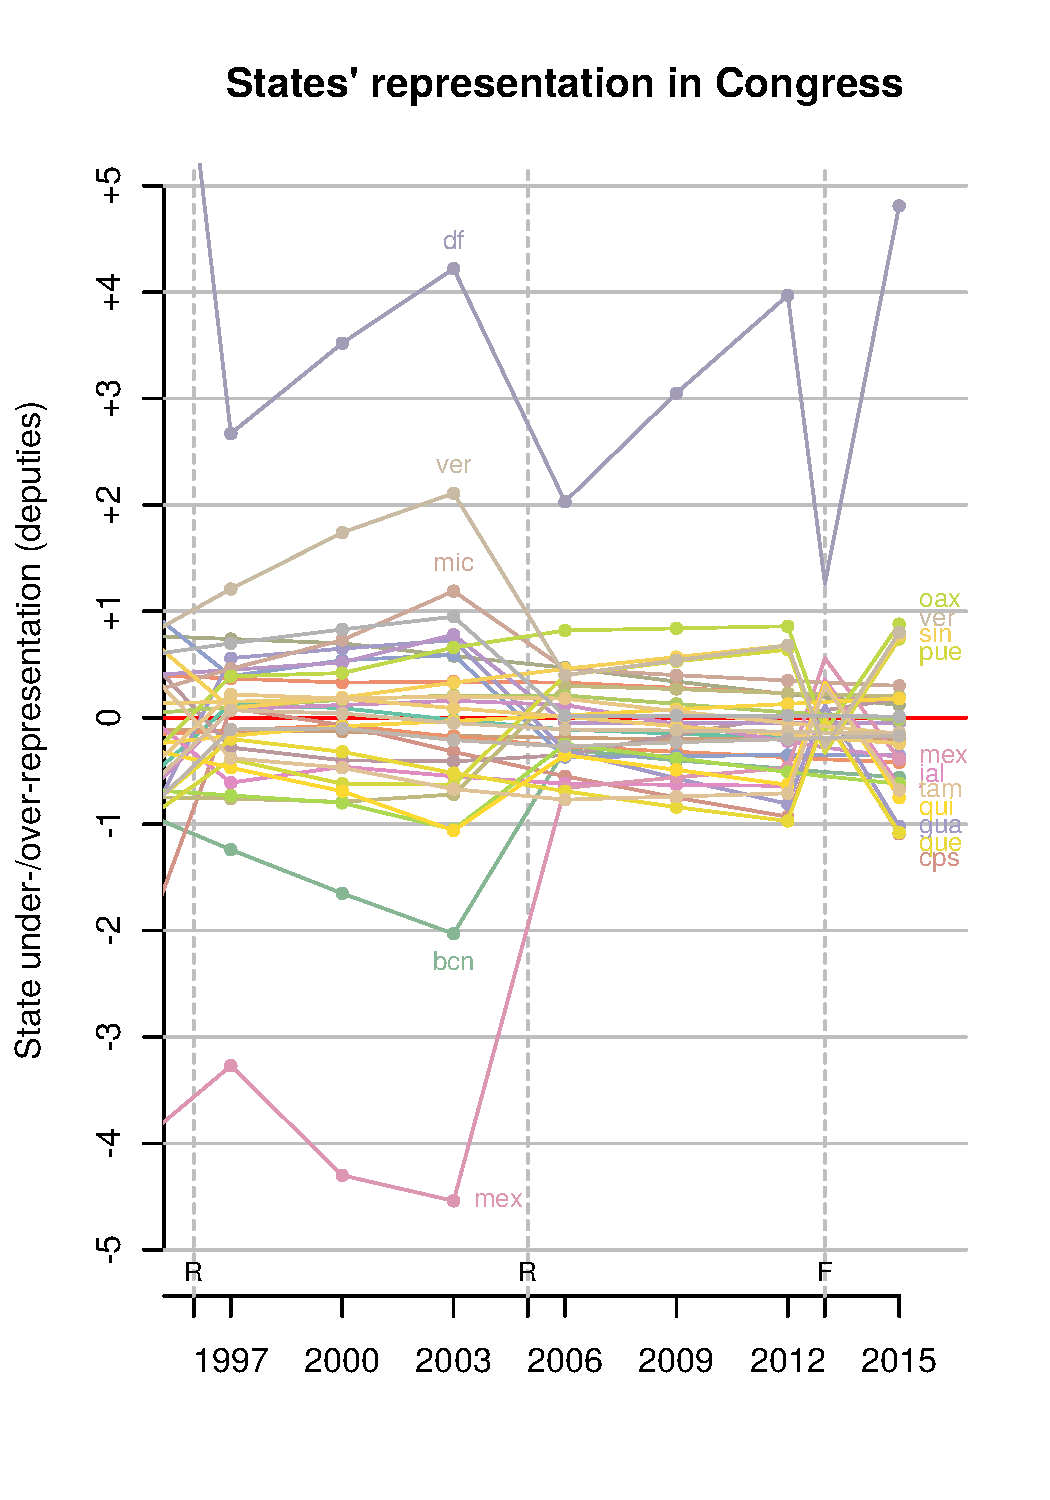
\includegraphics[width=.45\columnwidth]{statesUnderOverRep.pdf} & 
    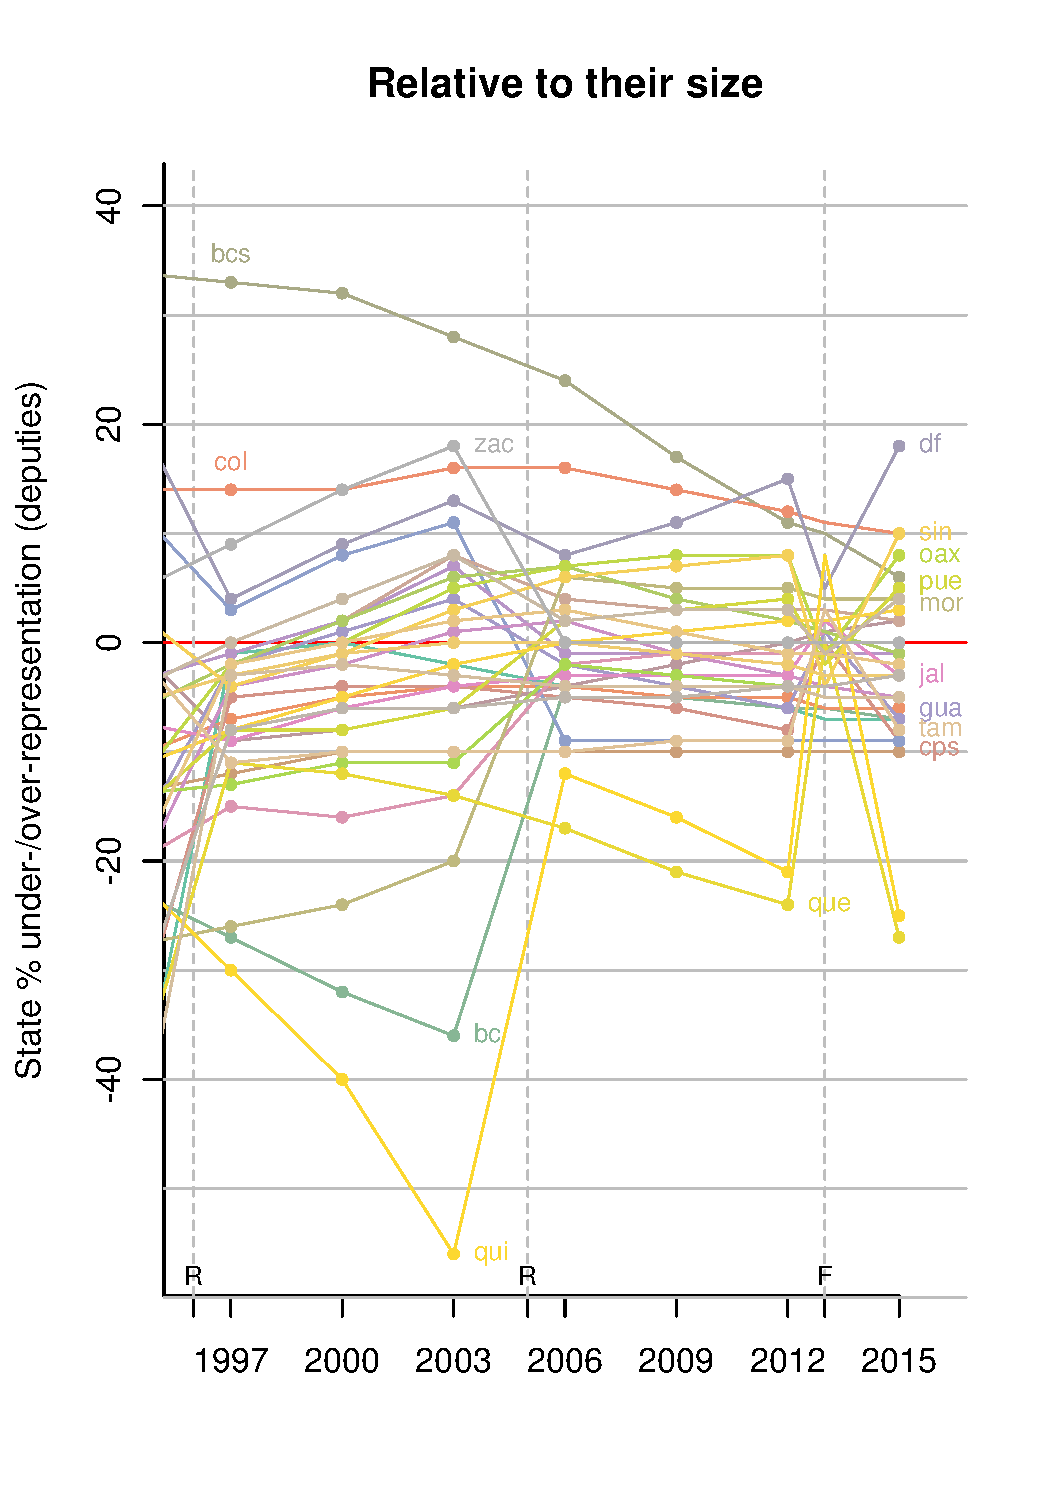
\includegraphics[width=.45\columnwidth]{statesUnderOverRep-rel.pdf} \\ 
  \end{tabular}
  \caption{Demography and state apportionment. Lines connect the lower chamber seats aportioned to seats due difference for each state over time. Letters R in the horizontal axis indicate redistricting, letter F a failed redistricting attempt (reporting the effect it would have had).}\label{F:underOverRep}
\end{center}
\end{figure}

Figure \ref{F:underOverRep} summarizes state's representation in Congress. We estimated each state's population at the time of each federal election since 1997. Estimation between 1997 and 2010, inclusive, relied on linear interpolation of the lustra census populations,\footnote{The years 1995 and 2005 had population counts, 2000 and 2010 had general censuses. The former collect much fewer attributes than the latter.} and linear extrapolation for 2012 and 2015. With moving population estimates, a time-series of states' fair share of congressional seats was computed (time-varying $Q$s). The actual number of seats apportioned is subtracted, yielding the state's over- or under-representation at the time of the election. A state with perfect apportionment in every election would appear as a flat, horizontal line at zero in the Figure. The left panel reports this measure in absolute terms (so that $+5$ indicates a state with five deputies more than its fair share), the right panel relative to seats apportioned to the state ($+5$ indicates five percent more deputies than its fair share).  

Since the first term of the subtraction is a real number and the second an integer, a fraction is bound to remain. Fractions in well-apportioned systems should all be less than 1 in absolute value---once that mark is passed, a full quota is reached, and a deputy is added or subtracted. The left panel shows that this is mostly the case for Mexico, but exceptions are, and have always been present. It is also plain that the 2006 map corrected, to some extent, important distortions that the 1997 map had failed to rectify. Under-representation of Baja California, but especially of the Mexico State dropped from two and five deputies less than due (deficits of 30 percent and less than 10 in relative terms), respectively, to near parity. Over-represented Veracruz behaved near symmetrically to Baja in absolute terms (not relative). And a distortion strongly favoring the Federal District ($+4$ deputies) was somewhat attenuated in 2006, but never removed. 

Persitent malapportionment is explained, in small part, by the allocation of two seats to small states. Relative over-representation of tiny Southern Baja and Colima was substantial, but only until recently. Population growth has made both worth their congressional seats. Yet relative over-representation remains substantial in migrant-worker-exporter Zacatecas up to 2003, and in the Federal District of late. Both states have lost population fast relative to the rest, and the system's design makes rapid demographic shifts slip away from grip. 

When redistricting plans are drawn, malapportionment does not exist \emph{de jure}. It exists \emph{de facto}. Mexico's constitution provides that every redistricting process must rely on the most recent population census available, with no attempt to estimate population change since (and, unlike the U.S., no obligation to redistrict as soon as a new census is available). Nor does it contemplate the use of lustrum counts instead. As a results, the redistricting process has built-in features explaining the persistence of malaportionment---what \citet{johnston.2002} calls ``creeping malapportionment'', whereby changes in constituency size over time create smaller seats. Compared to the 2000 census populations used for the 2006 map, the projection of 2000--2005 state population shifts are off by 9.7 percent on average, with a standard deviation of 6.9 percent. %The 2000--2005 population shifts projected to the year 2006, for instance, resulted in mean state populations deviating 9.7 percent compared to the census, with a standard deviation of 6.9 percent. 


With this in mind, it is puzzling that the redistributive nature of apportionment has not pushed for the adoption of alternative methods. The seventeen states that were under-represented in 2006 jointly controlled a majority (162) of single-member districts; fourteen of them have always been below the red line indicating fair representation. Does malapportionment have political consequences?

\subsection{Within states}

Despite automation and straightforward, formal redistricting criteria, Mexican parties in general, and IFE in particular, have been remarkably tolerant to unequally sized districts. This form of malapportionment is related in some degree to state imbalance in Congress, which perforce creates size differences across states' districts. But size inequality within states is also prevalent and substantial. 

Small deviations around a state's mean district population are unavoidable. But what constitutes a small deviation is hard to define. Courts in the U.S.\ have struck down district maps bearing less than 1\% differences without proper justification \citep{tuckerApportionment.1985}. Redistricting authorities generally view a \emph{de minimus} population deviations of as little as one or zero persons between congressional districts as desirable to inoculate against litigation. In stark contrast, IFE has considered deviations between 10 (in 2006) and 15\% (in 1997 and 2015) above or below mean state district size perfectly normal. Within such spread, a district at the bottom end is worth one-third more in Congress than another at the top end. Surprisingly, no party has ever challenged this in Court. 

The measure of malapportionment hinted bears relation to the relative representation index \citet{ansolabehere.gerber.snyderCourtRedis2002}. The $RRI$ was originally devised to measure how well are represented counties (some of which have several districts) in U.S.\ state assemblies. Focusing on districts instead, the index for a district $d$ belonging in state $s$ is

\begin{equation*}
RRI_{d,s} = \frac{1/population_d}{apportionment_s/population_s}
\end{equation*}

\noindent where the numerator is the the number of congressional seats per person in the district (the inverse of district $d$'s size) and the denominator is the average number of congressional seats per person in the parent state ($apportionment_s$ is the number of congressional seats awarded to state $s$). A district with unity index value has representation matching the `one person, one vote' ideal perfectly. Values above one indicate over-representation, values below one under-representation, and the measure is continous. An example shows how the index is interpreted. The number of congressional seats per person in district Ags-3rd in 2012 was about $1/300,000$. With three seats apportioned to the state of Aguascalientes and a total population of about 1,200,000, the district in question had 33 percent more representation than the state average, for an index value of 1.33. 

% year   min   .05  .25  .50  .75  .95  max 
% 2006  0.65  0.84 0.94 1.00 1.08 1.22 1.42 
% 2009  0.54  0.81 0.94 1.00 1.09 1.27 1.62 
% 2012  0.46  0.79 0.93 1.00 1.11 1.39 1.85 
% 2015  0.40  0.77 0.92 1.01 1.13 1.49 2.11 

\begin{figure}
\begin{center}
%    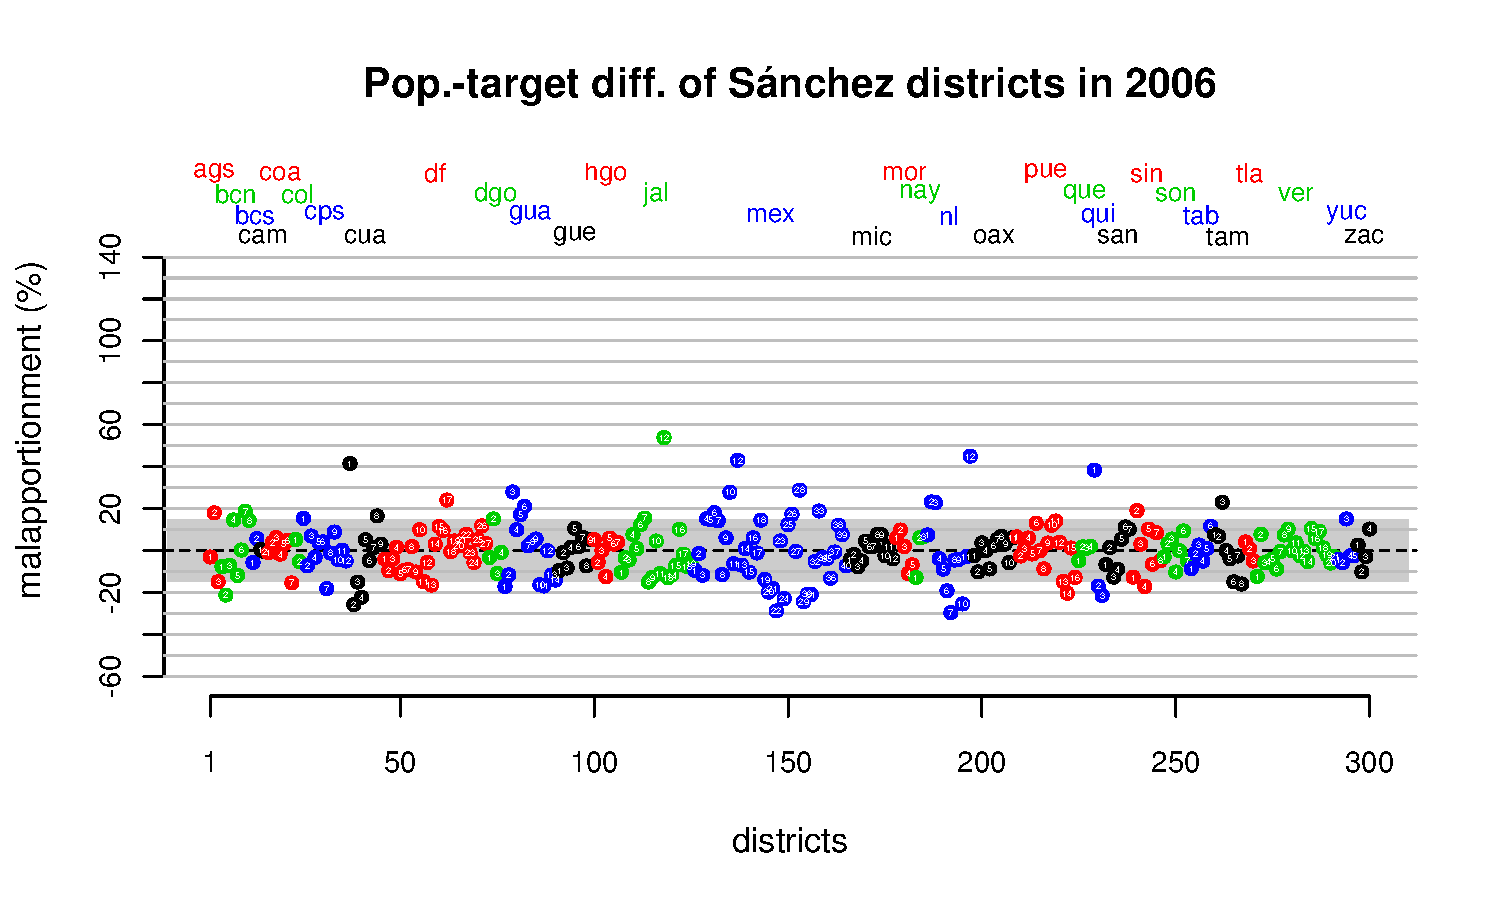
\includegraphics[width=.7\columnwidth]{malapp2006d0.pdf} \\
%    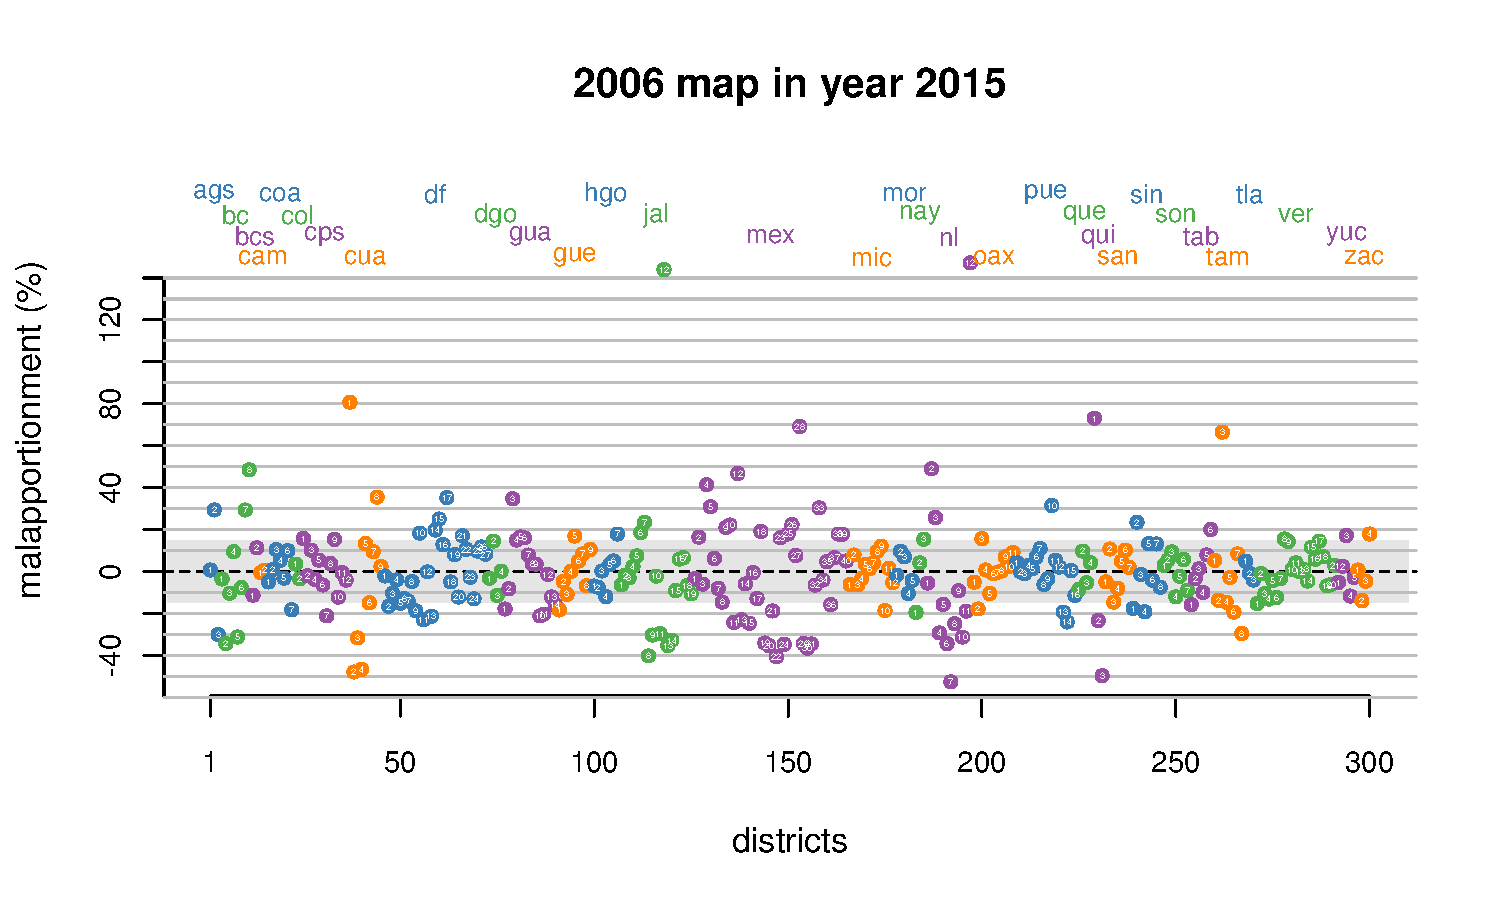
\includegraphics[width=.7\columnwidth]{malapp2015d0.pdf} \\
%    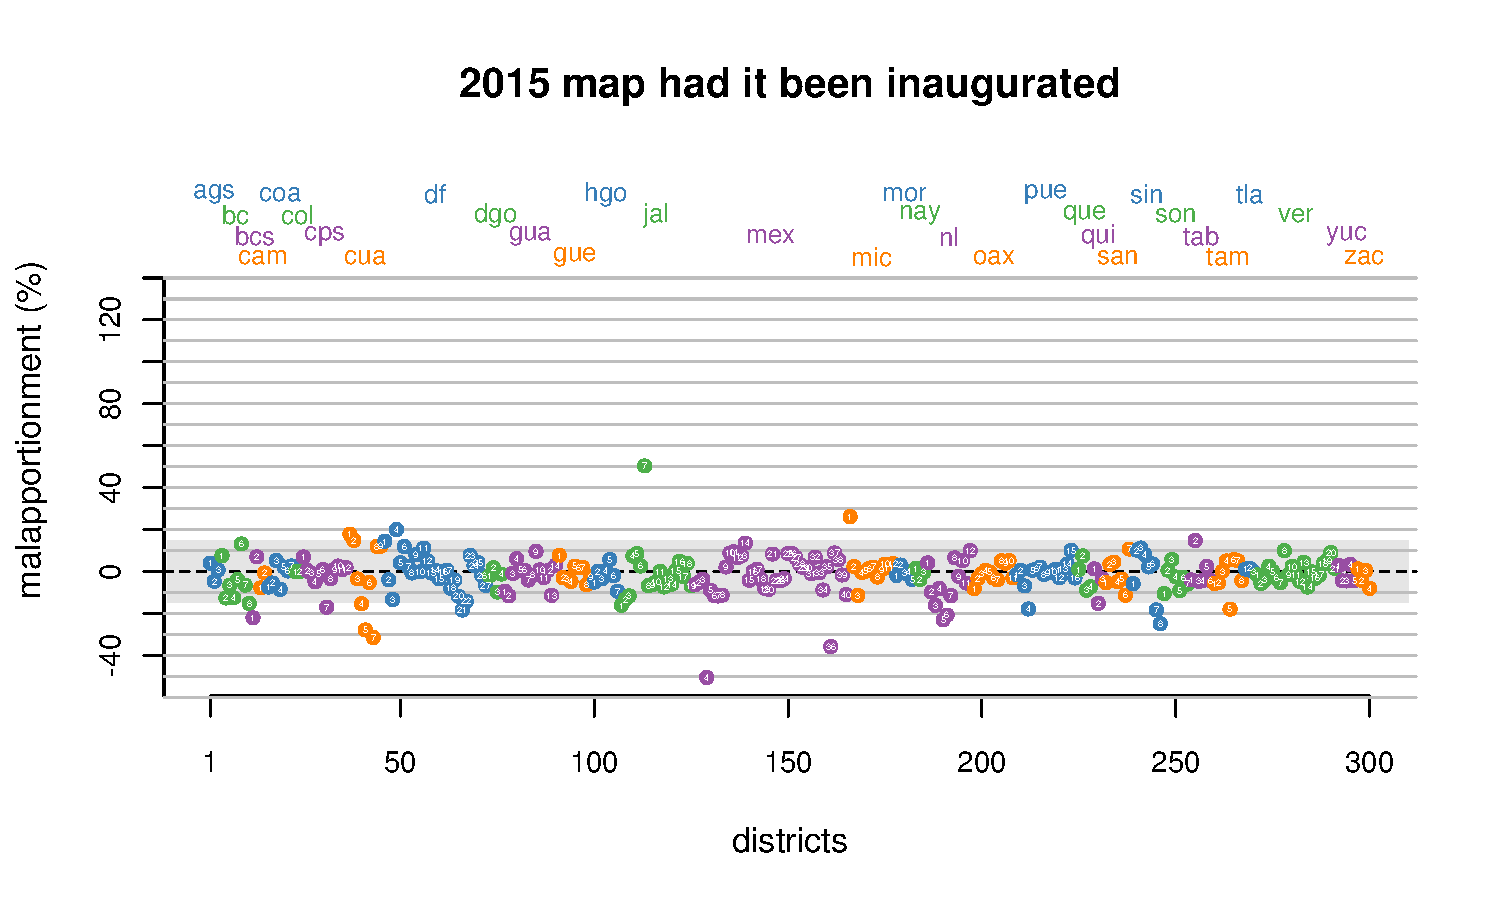
\includegraphics[width=.7\columnwidth]{malapp2015d3.pdf} \\
    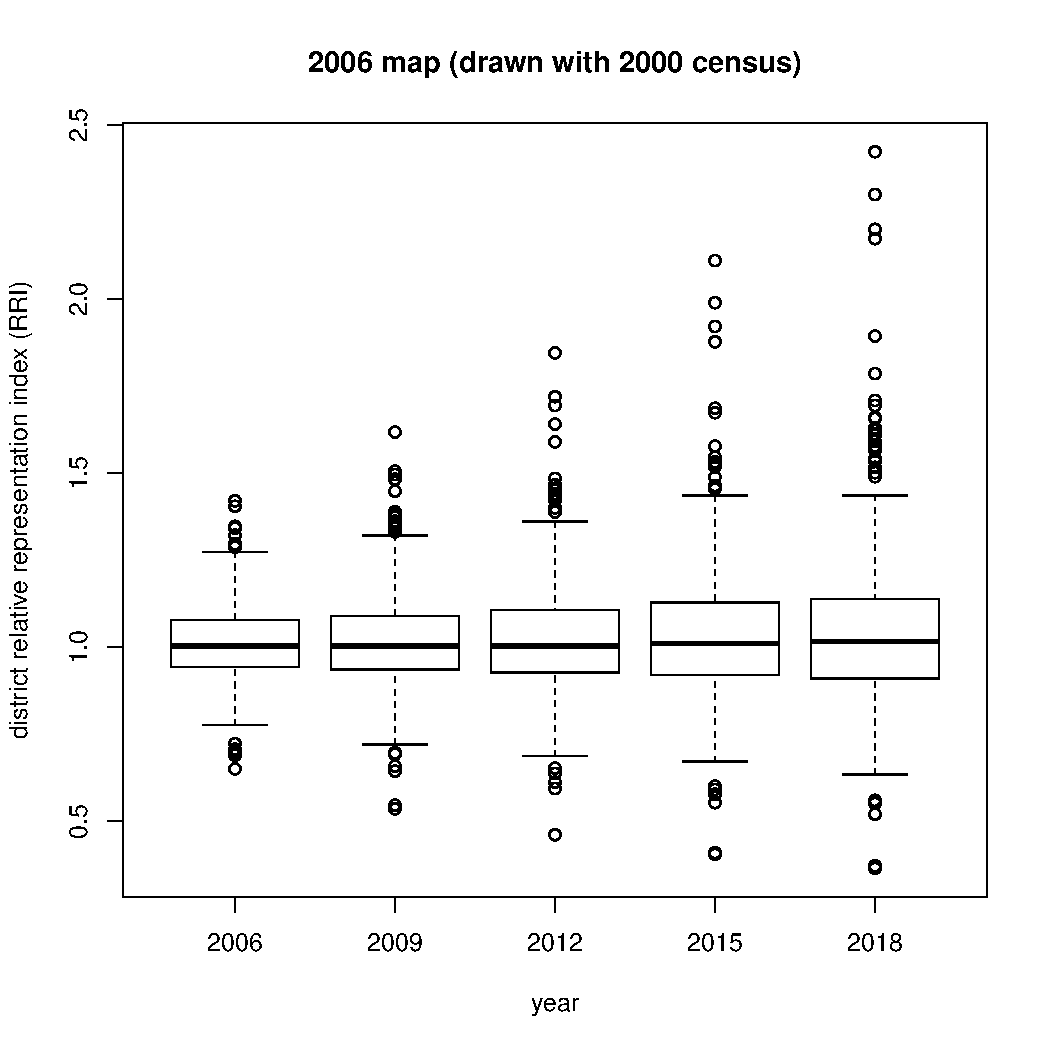
\includegraphics[width=.65\columnwidth]{rris0618d0.pdf} \\ 
    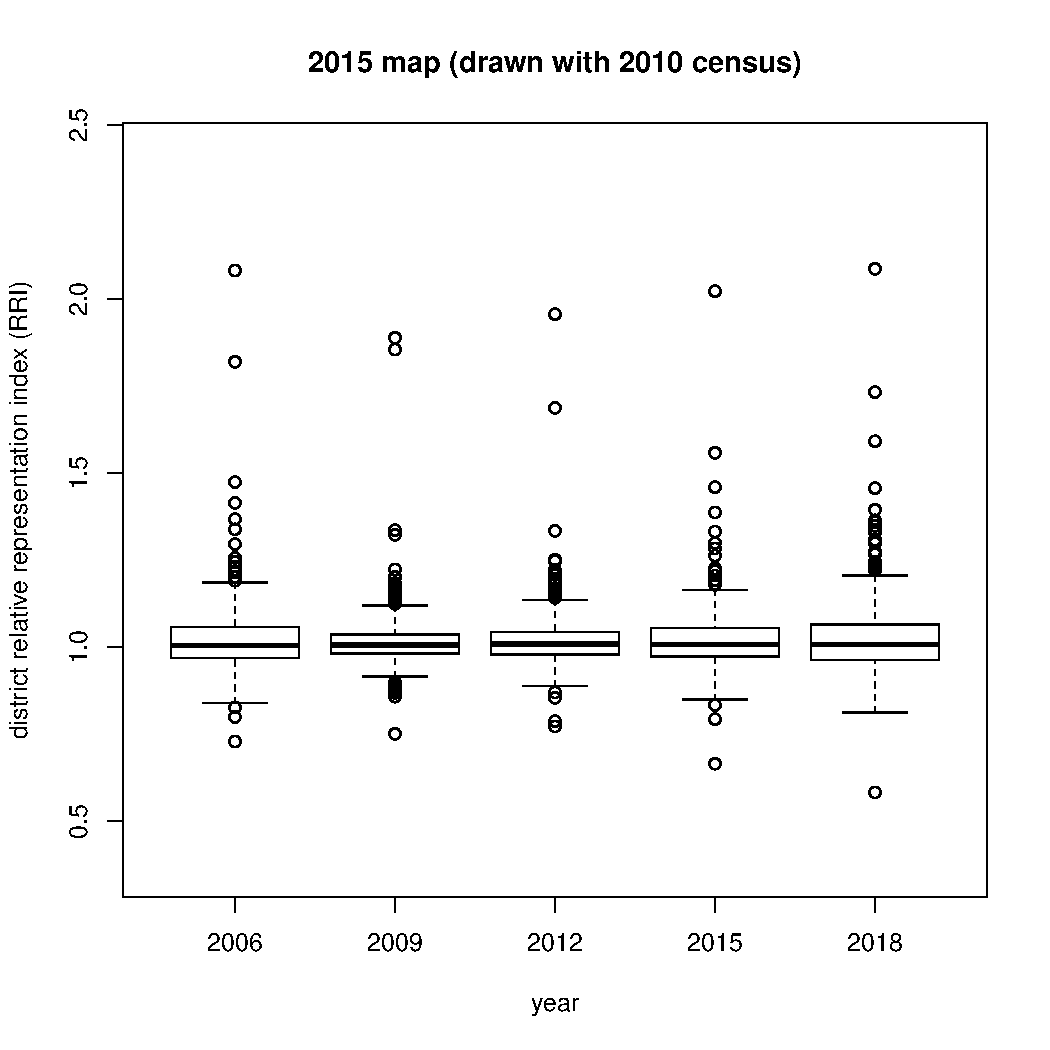
\includegraphics[width=.65\columnwidth]{rris0618d3.pdf}  
%    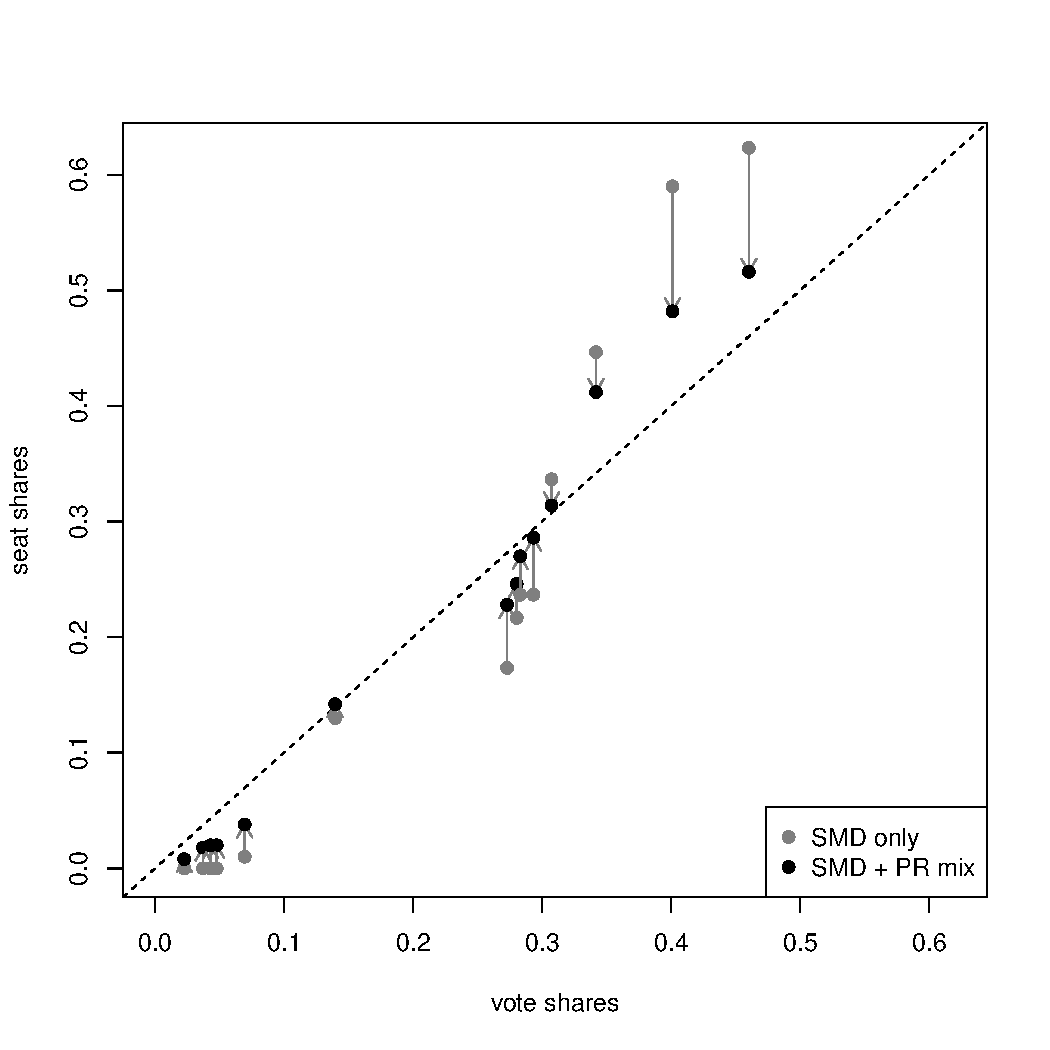
\includegraphics[width=.45\columnwidth]{votes-seatsSMDandMix0612.pdf} \\ 
%old  \caption{Malapportionment through years and maps. The $y$-scale measures district population relative to ideal (mean state population). The grey band is IFE's range of tolerance for district population imbalance ($\pm15\%$).}\label{F:malapp}
  \caption{Malapportionment through five elections and two maps. The top panel measures district representation in the 2006 map, the bottom in the 2015 (abandoned) map. Boxes cover the interquartile RRI range and include the median. Whiskers cover the upper and lower fences (excluding outlier districts). Yearly district populations are linear projections of the 2005 and 2010 censuses.}\label{F:malapp}
\end{center}
\end{figure}

Redistricting automation should make districts within states tend towards zero malapportionment. Population balance is, after all, the criterion that weighs more in the cost function. But this criterion weighs less than the others combined in the algorithm, and appears to be trumped rather easily. The preservation of municipal boundaries, for instance, is achieved by exploiting tolerated leeway. Figure \ref{F:malapp} shows how the imbalance tolerance band (in grey) is uniformly occupied by districts even right after a map's inception---in practice, the system does \emph{not} push towards perfect balance. And it is notable that when estimated population shifts are taken into account (as the plot does, unlike IFE), as many 16 percent of new 2006 districts were patently \emph{outside} the lax range of tolerance.\footnote{Census data reported at the electoral \emph{secci\'on} level are available since 2005 only. We projected the 2005--2010 changes to 2006 and 2015 for this exercise. Since so many districts are made of full municipalities, we could use that unit to extend it to 1997.} 

%Verify exactly how many district off the +/-15 band.

\begin{table}
\begin{center}
  \begin{tabular}{lrrrrr}
                 & \mc{5}{c}{Absolute malapportionment} \\
Map in year      & Min. & 1st quartile & median & 3rd quartile & max. \\ \hline
2006 map in 2006 & $<.01$ & 3.4 & 6.5 & 12.4 & 54.8 \\
2006 map in 2015 & .02 & 4.4 & 9.9 & 18.0 & 147.2 \\
2015 map in 2015 & .01 & 1.9 & 4.2 & 8.1 & 50.6 \\
  \end{tabular}
\caption{Changing malapportionment. For these statistics, each district's estimated population in 2006 and 2015 (from \emph{sección} 2005--2010 changes) is compared to its parent state's estimated mean district population.}\label{T:malap06inTime}
\end{center}
\end{table}

The requirement to keep municipalities with large indigenous population within the same district may also explain exceptions. As seen in Table \ref{T:malap06inTime}, median absolute district malapportionent of the 2006 map upon inauguration was 6.5\%, the third quartile surpassing the ten point tolerance margin (then used) at 12.4\% \citep[also,][]{trelles.mtz.tesisItam.2007}. For next year's midterm election, the same descrepancies will be 9.9 and 17.9\%, respectively. The abandoned 2015 map proposal did a much better job upon inauguration, with median absolute district malapportionment of 4.2\% and third quartile at 8.1\%. 

%Variance between states' census populations and population estimates at the time of redistricting, discussed above, cannot be smaller when dealing with sub-state units used to prepare districts, pushing about 80 new districts out of the broad $\pm 15$\% band. 

Whether districts below and above fair representation behave differently merits closer inspection. Whether due to technical difficulties or discretion, malapportionment may be the source of meaningful distortions in democratic representation. To which we now turn to. 

\section{Party Bias and Responsiveness}

This section estimates district responsivity and party bias---two effects of scholarly interest. M\'arquez (\href{http://bit.ly/1jgsQXE}{\url{http://bit.ly/1jgsQXE}}) has approached this theme using national national-level electoral data aggregates over two decades, uncovering a degree of responsivity characteristic of Westminster systems and party bias against the PAN under the status quo. We proceed with state-by-state breakdowns over much a shorter span (2006, 2009, and 2012). Doing so, much higher responsivity (owing to fewer districts, 9 by state on average) is uncovered, but no apparent party bias in neither the 2006 map nor 2015 proposals. 

\subsection{Systematic Bias}

\begin{figure}
\begin{center}
    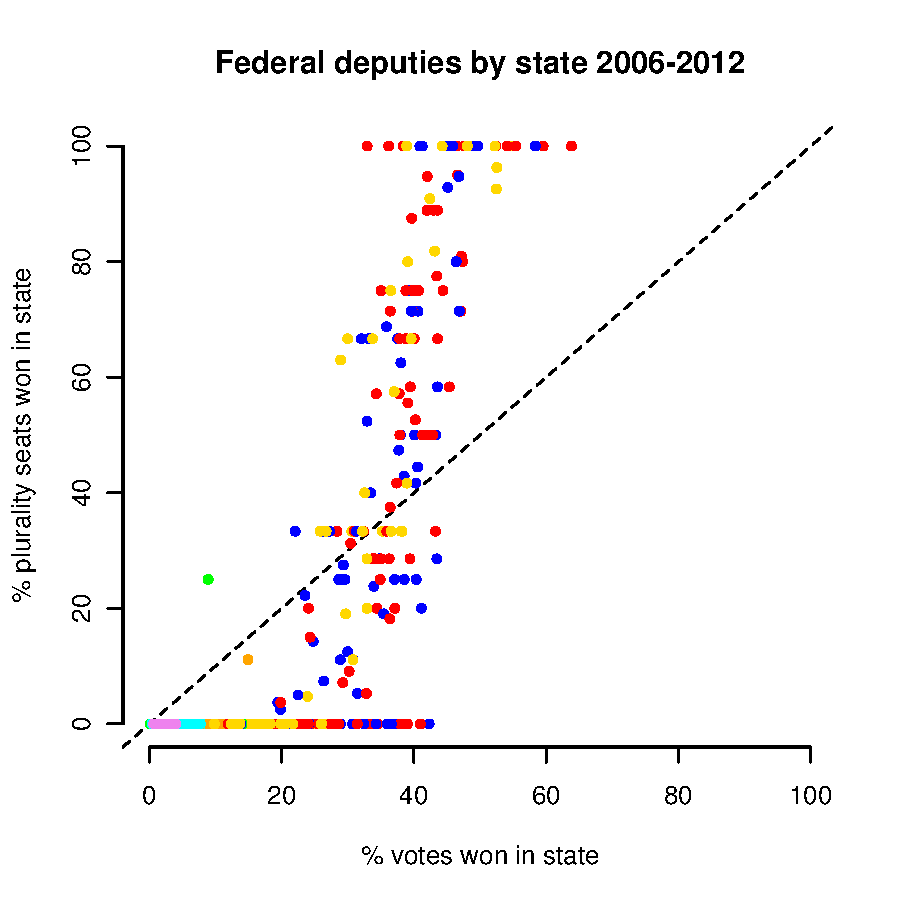
\includegraphics[width=.6\columnwidth]{resXedo20062012.pdf} 
\caption{Seats and votes in the states. Each point is a party-state-year, blue for PAN, red for PRI, gold for PRD, other colors for minor parties.}\label{F:seatsVotes}
\end{center}
\end{figure}

Consider now the relation between party votes and seats at the state level portrayed in Figure \ref{F:seatsVotes}. Each point reports the vote share that a party won in a state's federal deputy elections (x-axis) and the share of the state's congressional seats it received (y-axis). Colors distinguish the parties: PAN is blue, PRI is red, PRD is gold, Green is green, among others. For instance, the green dot floating to the left of the cloud is the Green party in Chiapas 2012, where it won 3 of 12 districts. The chart shows that 9 percent of the state's vote awarded the party 25 percent of the seats, an outstanding achievement for any party. The cloud manifests a steep upwards slope characteristic of first-past-the.post systems \citep{taagepera.CubeLaw.1973}.\footnote{Adding the excluded PR seats would level the slope considerably. Doing this would be easy with national aggregates. It is not evident how to carry it with state aggregates, since PR seats are awarded in five second-tier districts joining together several states each.} Points below the diagonal indicate under-representation, those above over-representation. There are notable differences among major parties: the PRI achieved over-representation in three-fifths of election-states between 2006 and 2012, the PAN in two-fifths, and the PRD in one-fourth only. 

With such setting, the possibility that districts are granting undue advantage to the PRI merits closer inspection. A priori, reasons to suspect IFE of cooking districts to favor one party or another are lacking. Major parties, after all, permanently influence the election regulator, ambition counteracting ambition \citep{estevez.magar.rosas.2008}. But that those who draw the district lines can distort a fundamental link of the democratic process is well established in the literature \citep{altman.mcdonald2011bard,cox.katz.2002,engstrom2006redisttrictApsr,rossiter.etal.1997,king.1990elRespBiasMultiparty,balinskiYoung2001FairRep,otero.2003}. Has the insidious gerrymandering reared its ugly head in Mexico? This section estimates majority and party effects in the proposed districts and the status quo. Majority effects are huge, partisan effects negligible. 

\subsection{Two Classes of Distortion}

Undue advantage is known, in the specialized literature, as partisan bias, and is one goal that strategic redistricters pursue. It is not, however, alone: scholarship highlights district responsiveness, also know as majoritarian bias, as another goal. These ought to be distinguished \citep[this paragraph draws heavily on][, ch.\ 3]{cox.katz.2002}. Partisan bias helps the beneficiary buy seats with fewer votes than others. Because seat distribution is a constant sum game, bias in favor of someone always implies bias against someone else. One way of introducing party bias in district lines is with the conventional redistricting strategy known as packing: group your adversary's voters in few districts, wasting votes to win unnecessarily safe seats, raising the price of victory. Responsiveness, on the other hand, is the feature granting a seat bonus to large parties. Maximal responsiveness occurs within each single-member district in isolation: the winner takes all, the rest nothing. The same could be achieved in a whole state by drawing lines so that every district is representative of the state's electorate (Cox and Katz's microcosm strategy). The party with most votes wins every seat, maximizing the vote responsiveness of the proposal. 

Formalizing party bias and responsiveness opens the way towards estimation of these district characteristics. The two-party case is simpler and extends to multiparty systems \citep{taagepera.CubeLaw.1973,tufte1973seatsVotes,king.browning1987biasRespUS}. It is a generalization of the cube law stipulating that 

\begin{equation}
 \frac{s}{1-s} = e^\lambda *  \left(\frac{v}{1-v}\right)^\rho \iff
 \texttt{logit}(s) = \lambda + \rho *  \texttt{logit}(v)
\end{equation}\label{E:cubeLaw}

\noindent where $s$ is the seat share that party 1 won with vote share $v$; $\lambda$ is party 1's bias relative to party 2 (positive values favor party 1, negative values favor party 2); and $\rho$ is the districts' responsiveness. With $\lambda=0$ a system with no party bias ensues. Figure \ref{F:lambdaRhoEx} shows how the parameters affect the vote-to-seats conversion. 

% comment [Mike] how do multiple parties affect bias/responsiveness estimates, compared to two-party setting? I would expect that a party would often need less than 50% of the vote to win 50% of seats due to many parties receiving votes in single-member districts.

\begin{figure}
\begin{center}
    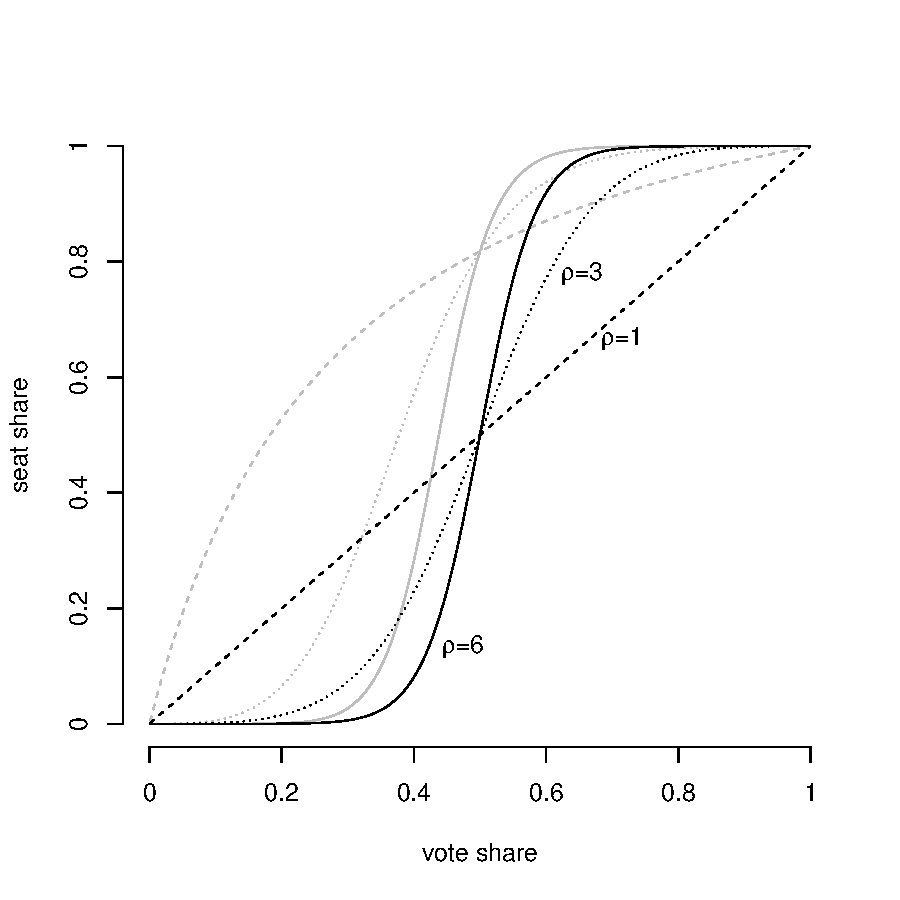
\includegraphics[width=.55\columnwidth]{rhoExample.pdf} 
\caption{Illustration of estimated parameters. Party bias is set to $\lambda=0$ in non-grey lines. Grey lines replicate the colored ones with $\lambda=+1.5$.}\label{F:lambdaRhoEx}
\end{center}
\end{figure}

Non-grey lines lack party bias to illustrate variable responsiveness. A system with $\rho=1$ is perfectly proportional representation, the ideal type against which the evaluation of real districts are often contrasted. It appears as the dotted green diagonal: every party winning $x$\% of the vote gets, precisely, $x$\% of seats. $\rho=3$ characterizes the classic cube law, the red curve over-representing the winner (points above the diagonal). Here a party with 55\% of the vote earns two-thirds of the seats, but with 33\% it earns only one-tenth of the seats. As responsivity grows, the curve gets steeper, until barely crossing the majority threshold suffices to win all the available seats. 

Grey lines replicate the values of $\rho$ just discussed but with $\lambda = 1.5$ added. Bias in favor of the party produces a leftward pull of lines. In other words, a bias-favored party requires less effort to reach the threshold for large-party over-representation. (The grey dotted line demonstrates how, due to logit links in Equation 1, party bias also reshapes the function's trace.)

A multiparty and estimable version of equation 1 \citep{king.1990elRespBiasMultiparty} establishes that party $j$'s ($j=1,2,\ldots,J$) expected seat share is 
\begin{equation}
 E(s_j) = \frac{e^{\lambda_j} * v_j^\rho}{\sum_{m=1}^{J} e^{\lambda_m} * v_m^\rho}
\end{equation}

\noindent with data and parameters indexed to identify the parties. \citep[Another, with application to Argentine federalism, is][.]{calvo.micozzi.govReform.2005} Setting $\lambda_2 = 0$, as done below, forces the remainder $\lambda_{j \neq 2}$ to express party bias with relation to the PRI's ($j=2$ for this party in the dataset). This is convenient to test the presumption of PRI-favoring bias:. if present, $\hat{\lambda}_{j \neq 2}<0$ would result.

A common estimation strategy relies on a time-series of national aggregates (this is what M\'arquez did for eight elections 1991--2012, uncovering substantive anti-PAN bias and high responsiveness). The estimation strategy here is with state-level data. One disadvantage of the approach is that states have few districts (9.4 on average), and this will amplify the system's responsiveness \citep{taagepera.CubeLaw.1973}. The advantages are many. The approach multiplies observations. This is evident in Figure \ref{F:seatsVotes}, with many points despite reporting three elections only. It holds the actual district structure constant---redistricting in 1997 and 2006 invalidates district comparability before and after. And it takes advantage in the variation of state party systems (this draft fails to take full advantage of this variance, but this could be exploited further). 

\begin{figure}
\begin{center}
  \begin{tabular}{cc}
    (a) & (b) \\
    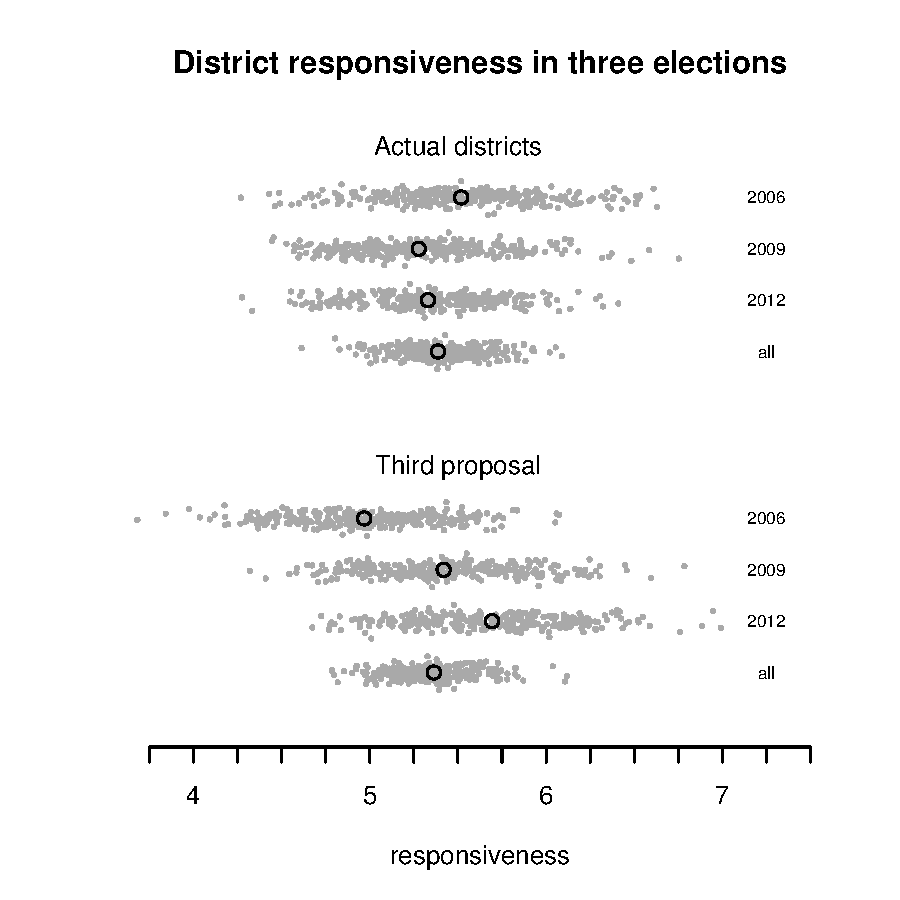
\includegraphics[width=.45\columnwidth]{resp200612s0s3.pdf} &
    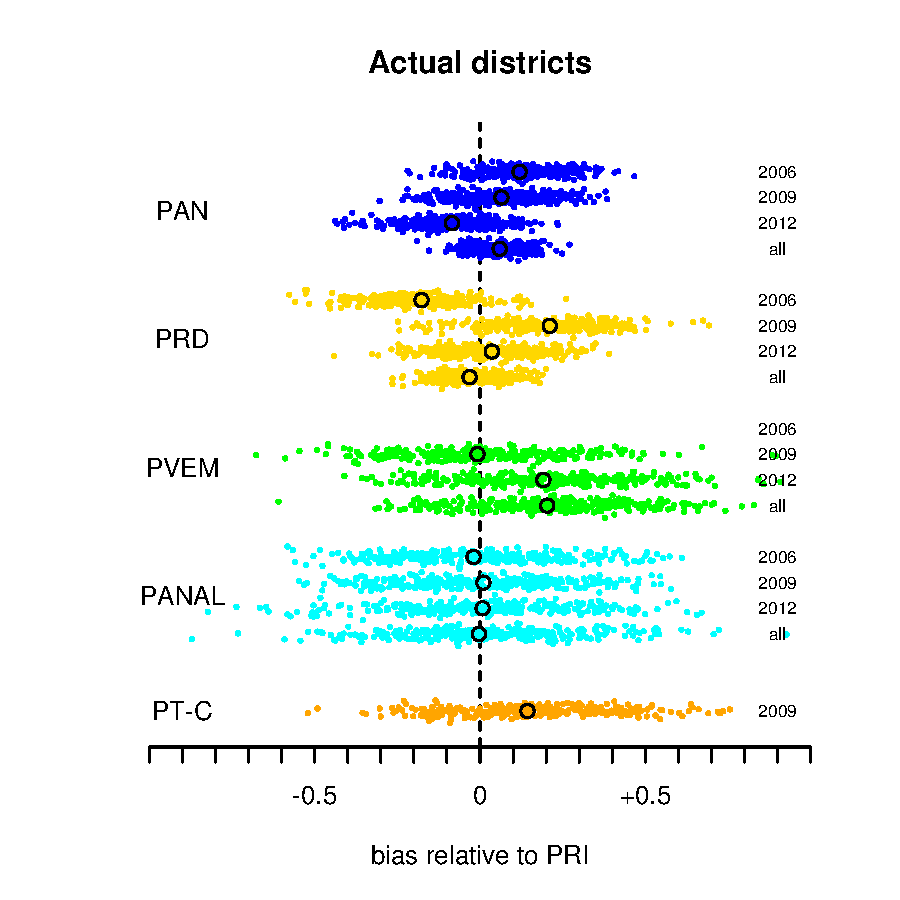
\includegraphics[width=.45\columnwidth]{bias200612s0.pdf} \\
    (c) & (d) \\
    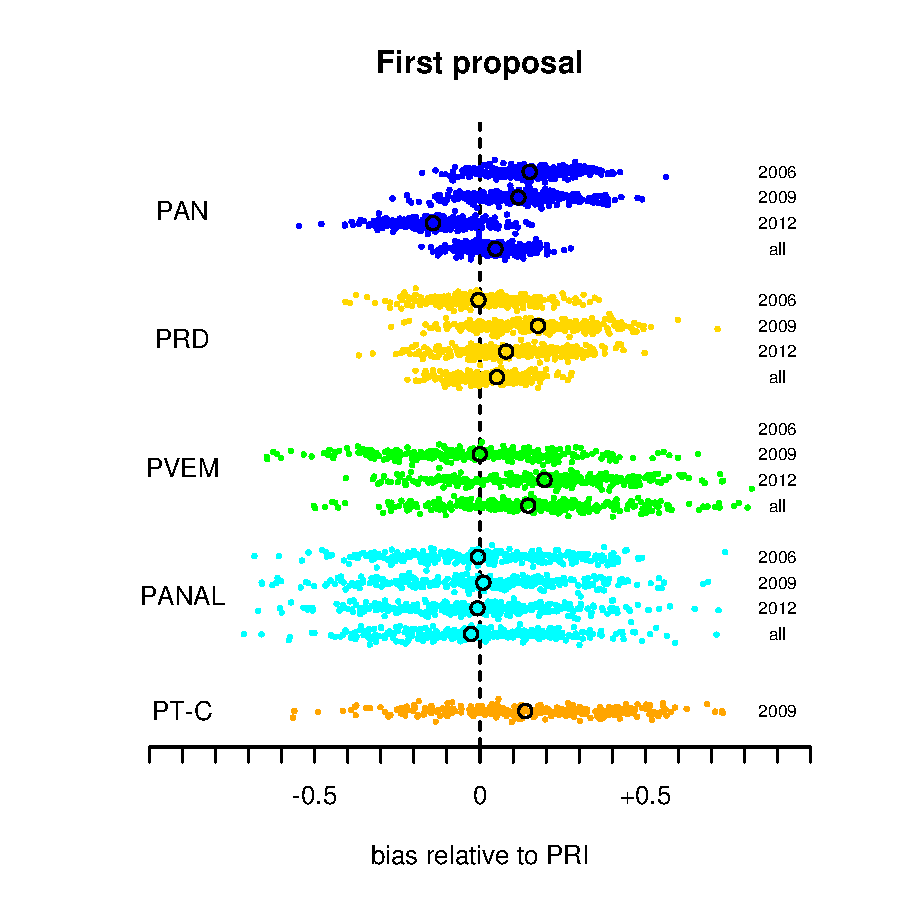
\includegraphics[width=.45\columnwidth]{bias200612s1.pdf} &
    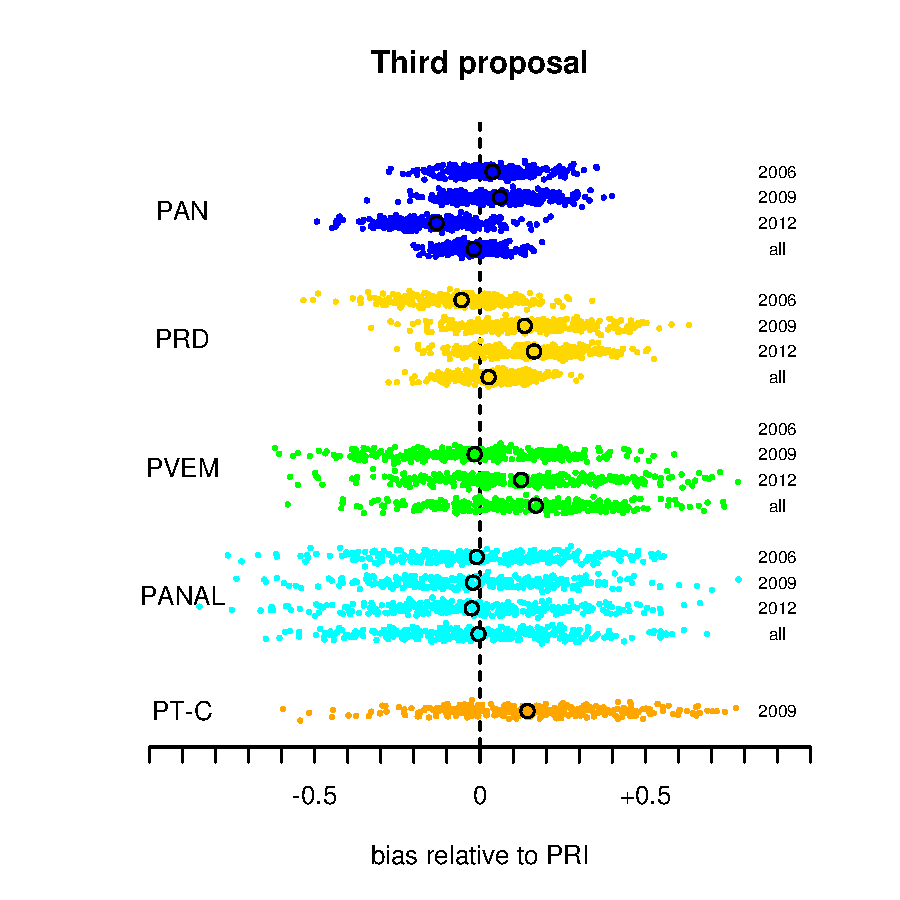
\includegraphics[width=.45\columnwidth]{bias200612s3.pdf} 
  \end{tabular}
  \caption{Redistricting, responsiveness, and party bias. Plots report the posterior sample of model's parameters $\lambda_j$ for four parties and $\rho$, and the median value (black circles).}\label{F:posterior_s0s1s3}
\end{center}
\end{figure}


The  method of estimation is MCMC \citep{jackman.2000}.\footnote{Three chains were iterated 10 thousand times, taking every fiftieth observation of the last 5 thousand to sample the posterior distribution. Convergence was gauged visually with traceplots of the separate chains for each of the model's parameters. Estimation performed with JAGS \citep{jags.cite}, implemented from R \citep{r.cite} using package R2jags \citep{r.r2jags}. Data and code to replicate the analysis can be found at HTTP...} As expected, district responsiveness is extremely high, between 5 and 6 depending on the year selected (the steepest line in illustrative Figure \ref{F:lambdaRhoEx} has $\lambda=6$). Figure \ref{F:posterior_s0s1s3}.a reports point estimates (the black circles are the median of the posterior sample of the responsiveness parameter) for each year separately, all years pooled together, and comparing actual districts to the first and third redistricting proposals. Estimate precision is assessed with the cloud of grey points (technically, it is the full sample of posterior $\rho$s). The redistricting proposal makes little change to district responsiveness, it just makes it slightly more volatile from one election to next. Owing to few districts per state, the estimated responsiveness at the state level ($\hat{\rho} \approx 5.5$) is twice M\'arquez's nationwide ($\hat{\rho} = 2.6$). All three parties experience situations of large party bonus and small party penalty that, to a good extent, cancel each other in the national statistic.

Regarding party bias, signals that are not weak all tend to be accompanied by a good deal of noise, with few exceptions. At the national level, and over a longer haul, M\'arquez discovers bias in favor of the PRI, but mostly in favor of the PRD, and against the PAN, that seems not the product of chance alone. Analysis at the state level reveals no such biases. As said, Figures \ref{F:posterior_s0s1s3}.b--d express bias relative to the PRI. Although PAN experienced weak signal in its favor in the whole 2006--12 period, a fair density of the blue cloud is, in fact, negative. PRD vs.\ PRI bias is clearly centered at zero in the full period. The left did experience significant bias in isolated years: against in 2006, in favor in 2009. Perhaps many voters who strategically abandoned the hopeless PRI presidential candidate in 2006 to vote for L\'opez Obrador did so in districts where PRI's congressional candidates still won. No other year for no other party reveals any bias unaccompanied by much noise.

% \section{Malapportionment and margin}

% \begin{figure}
% \begin{center}
%   \begin{tabular}{cc}
%     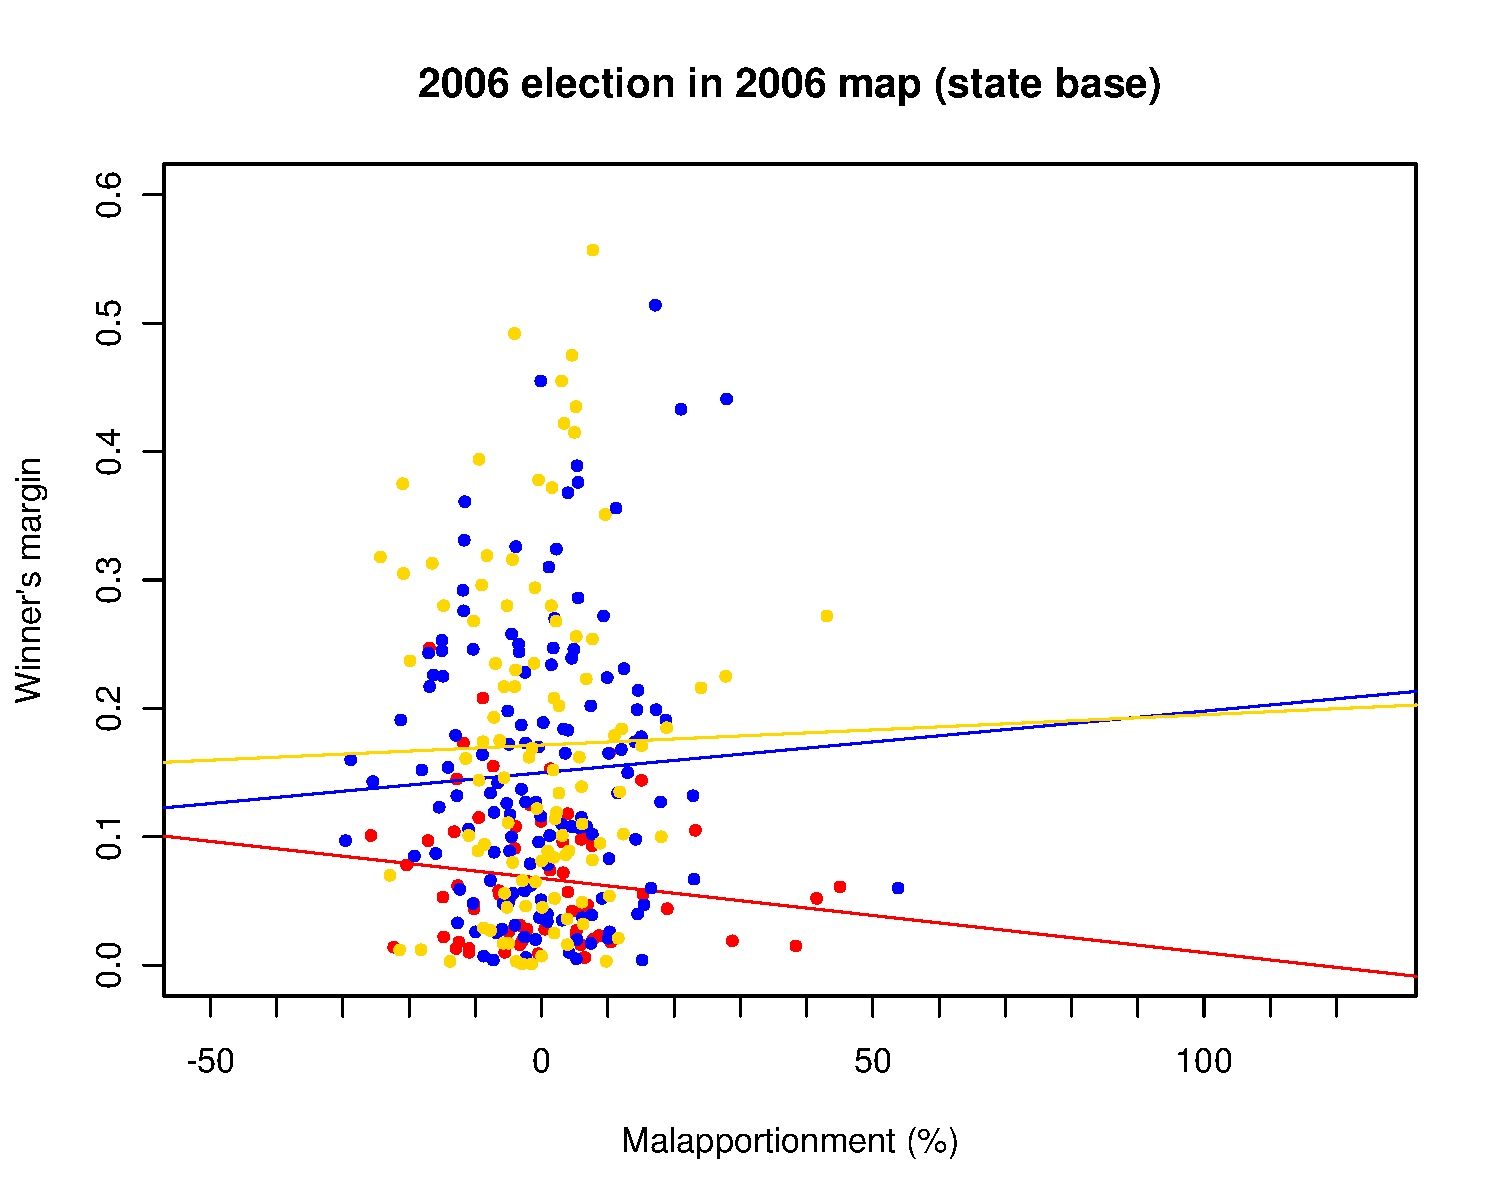
\includegraphics[width=.4\columnwidth]{malmg2006d0sta.pdf} & 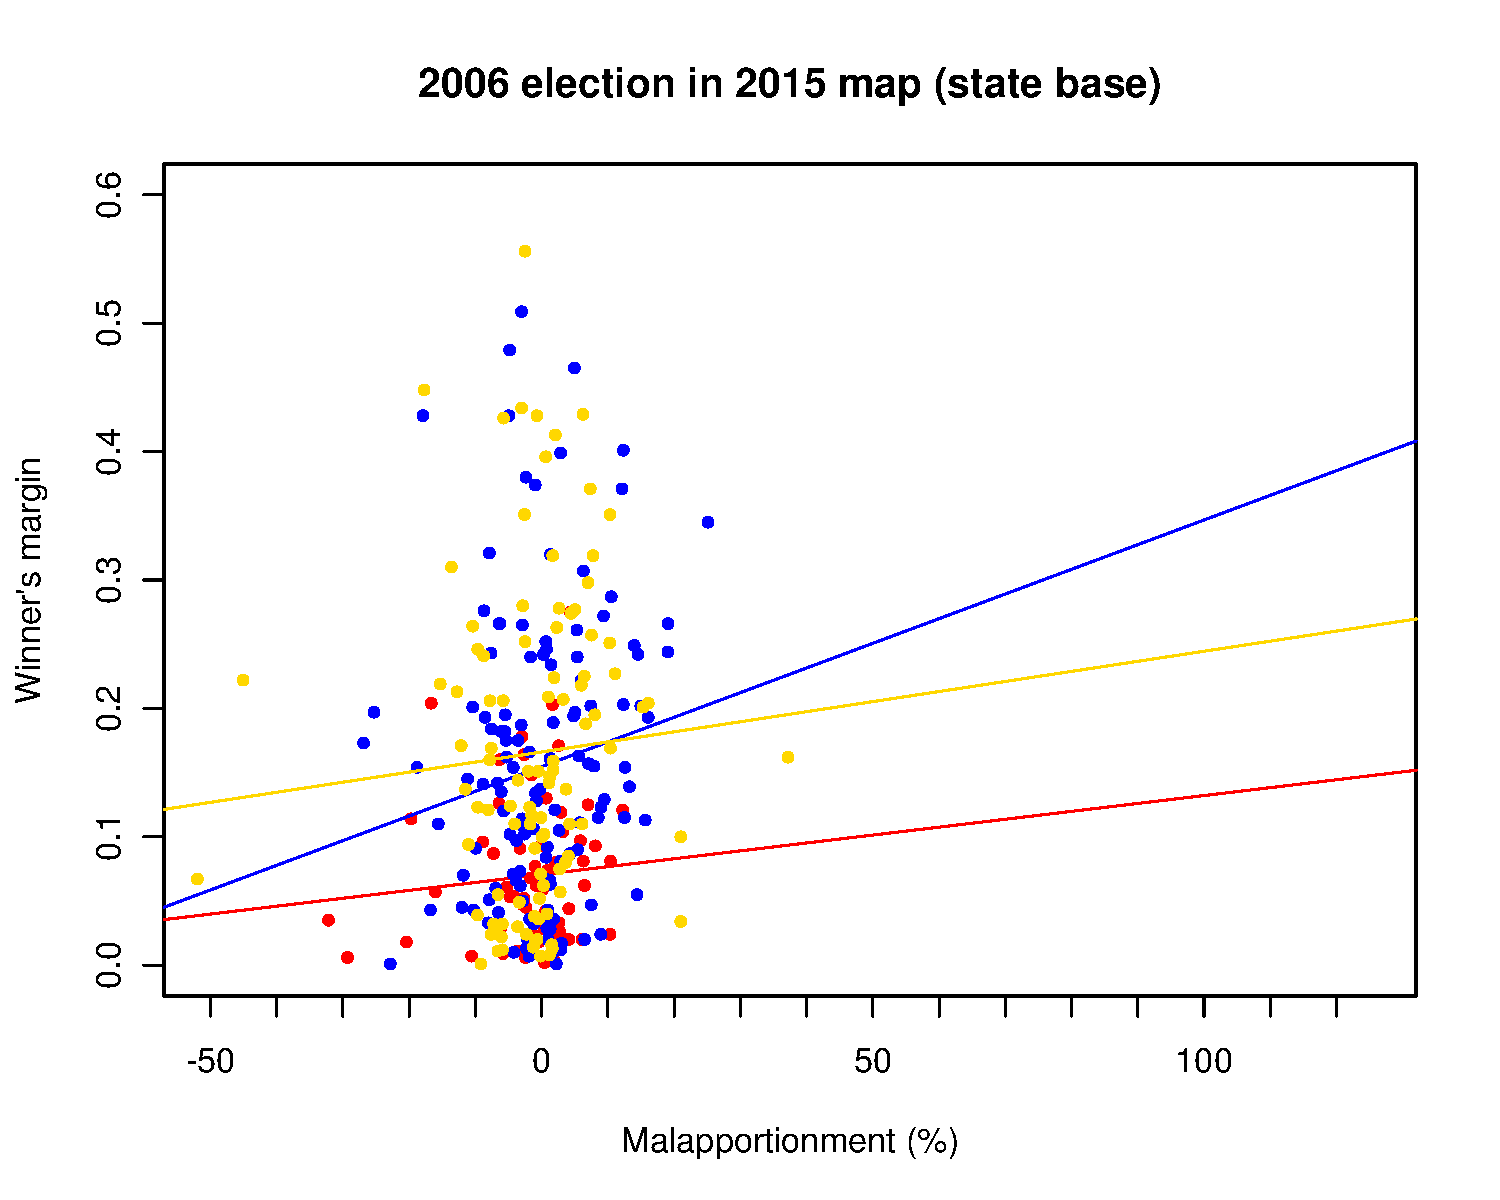
\includegraphics[width=.4\columnwidth]{malmg2006d3sta.pdf} \\
%     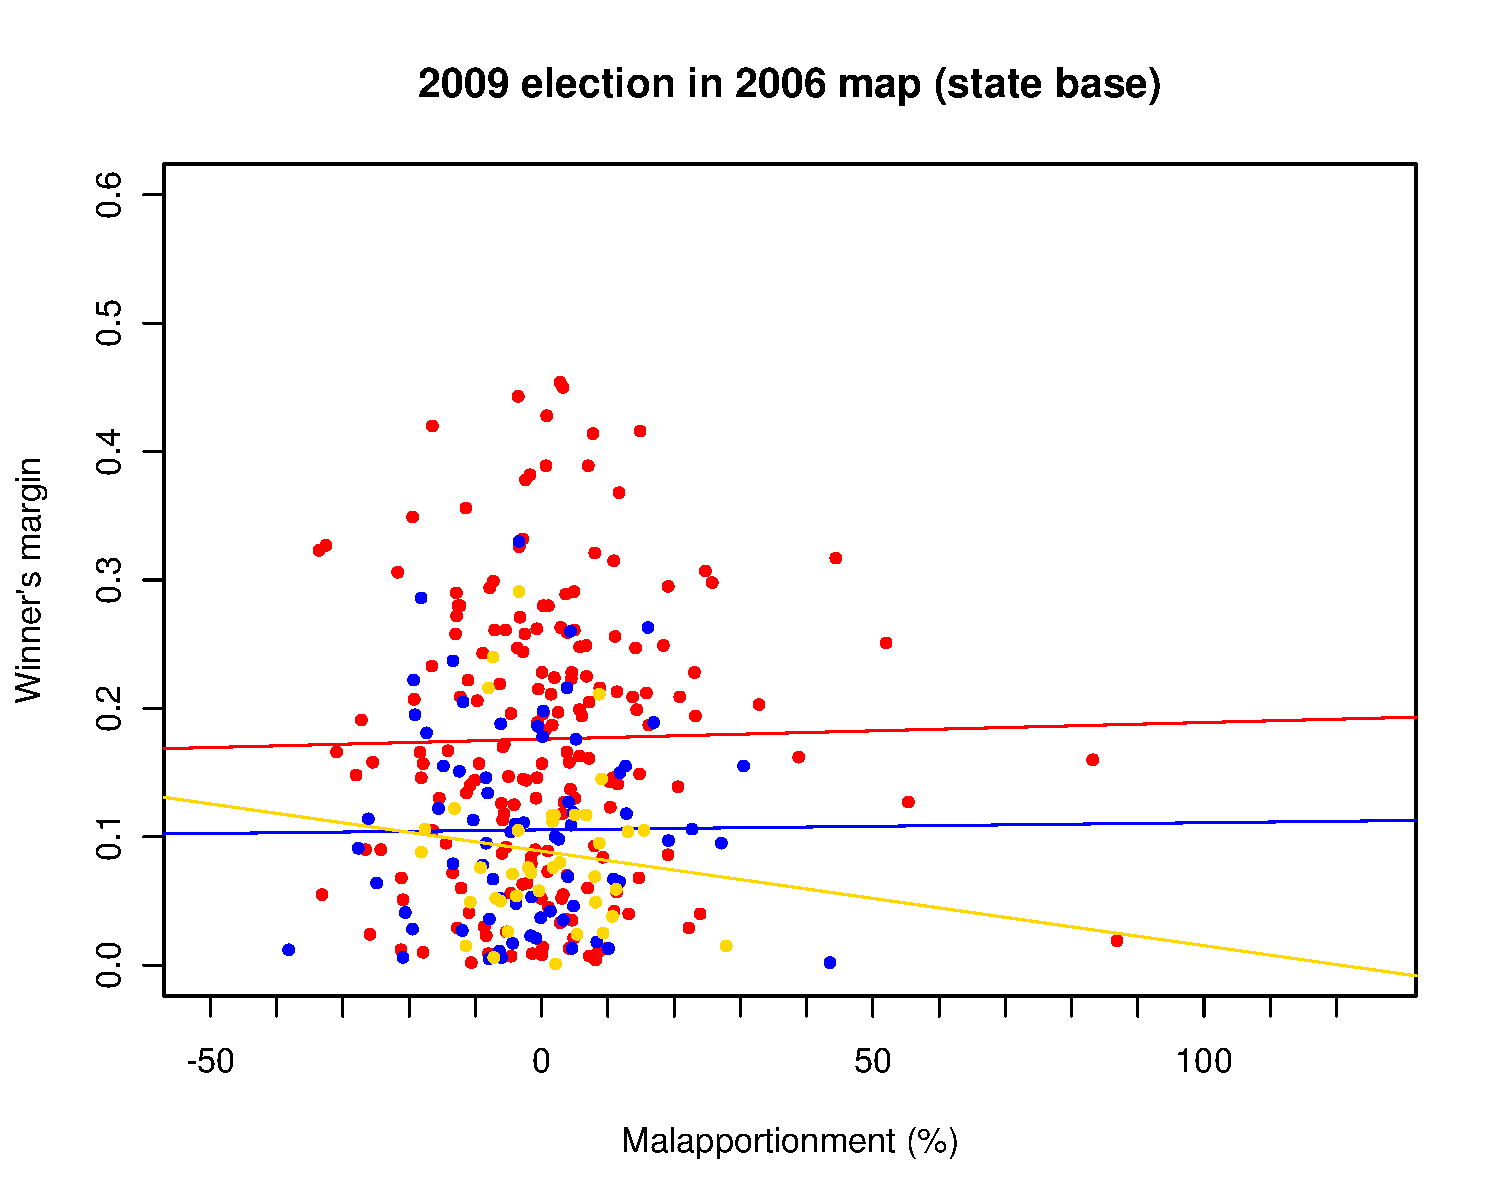
\includegraphics[width=.4\columnwidth]{malmg2009d0sta.pdf} & 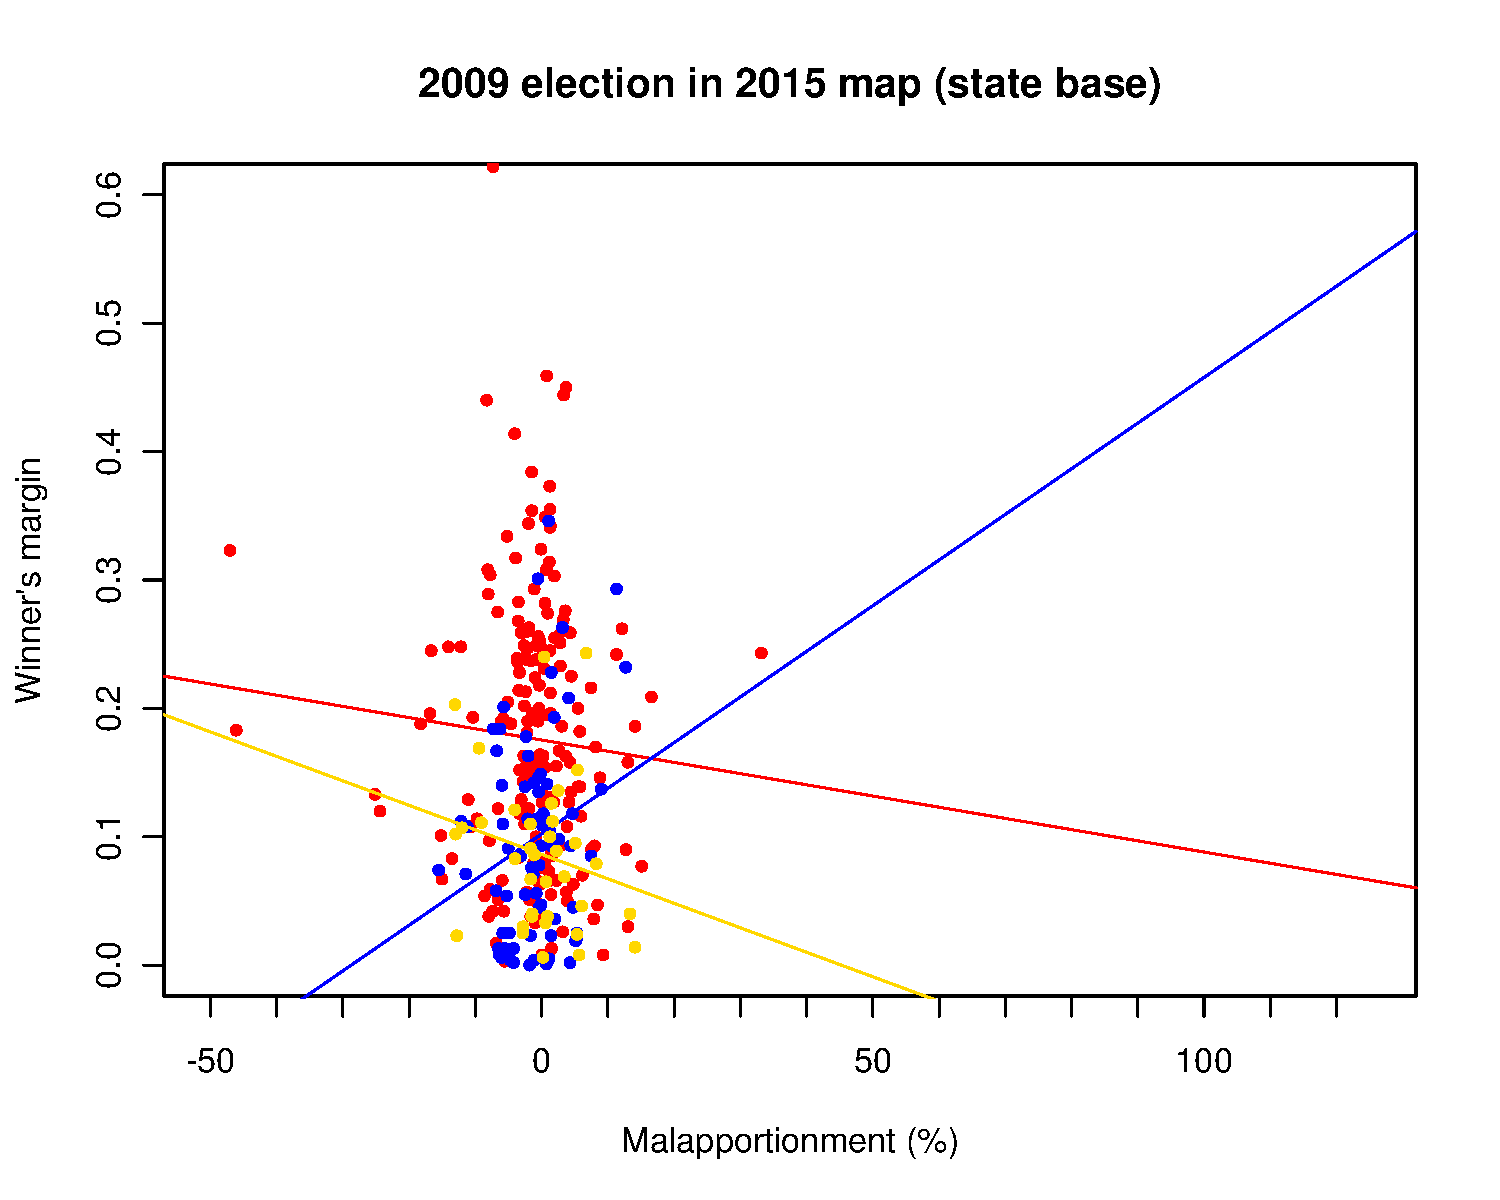
\includegraphics[width=.4\columnwidth]{malmg2009d3sta.pdf} \\
%     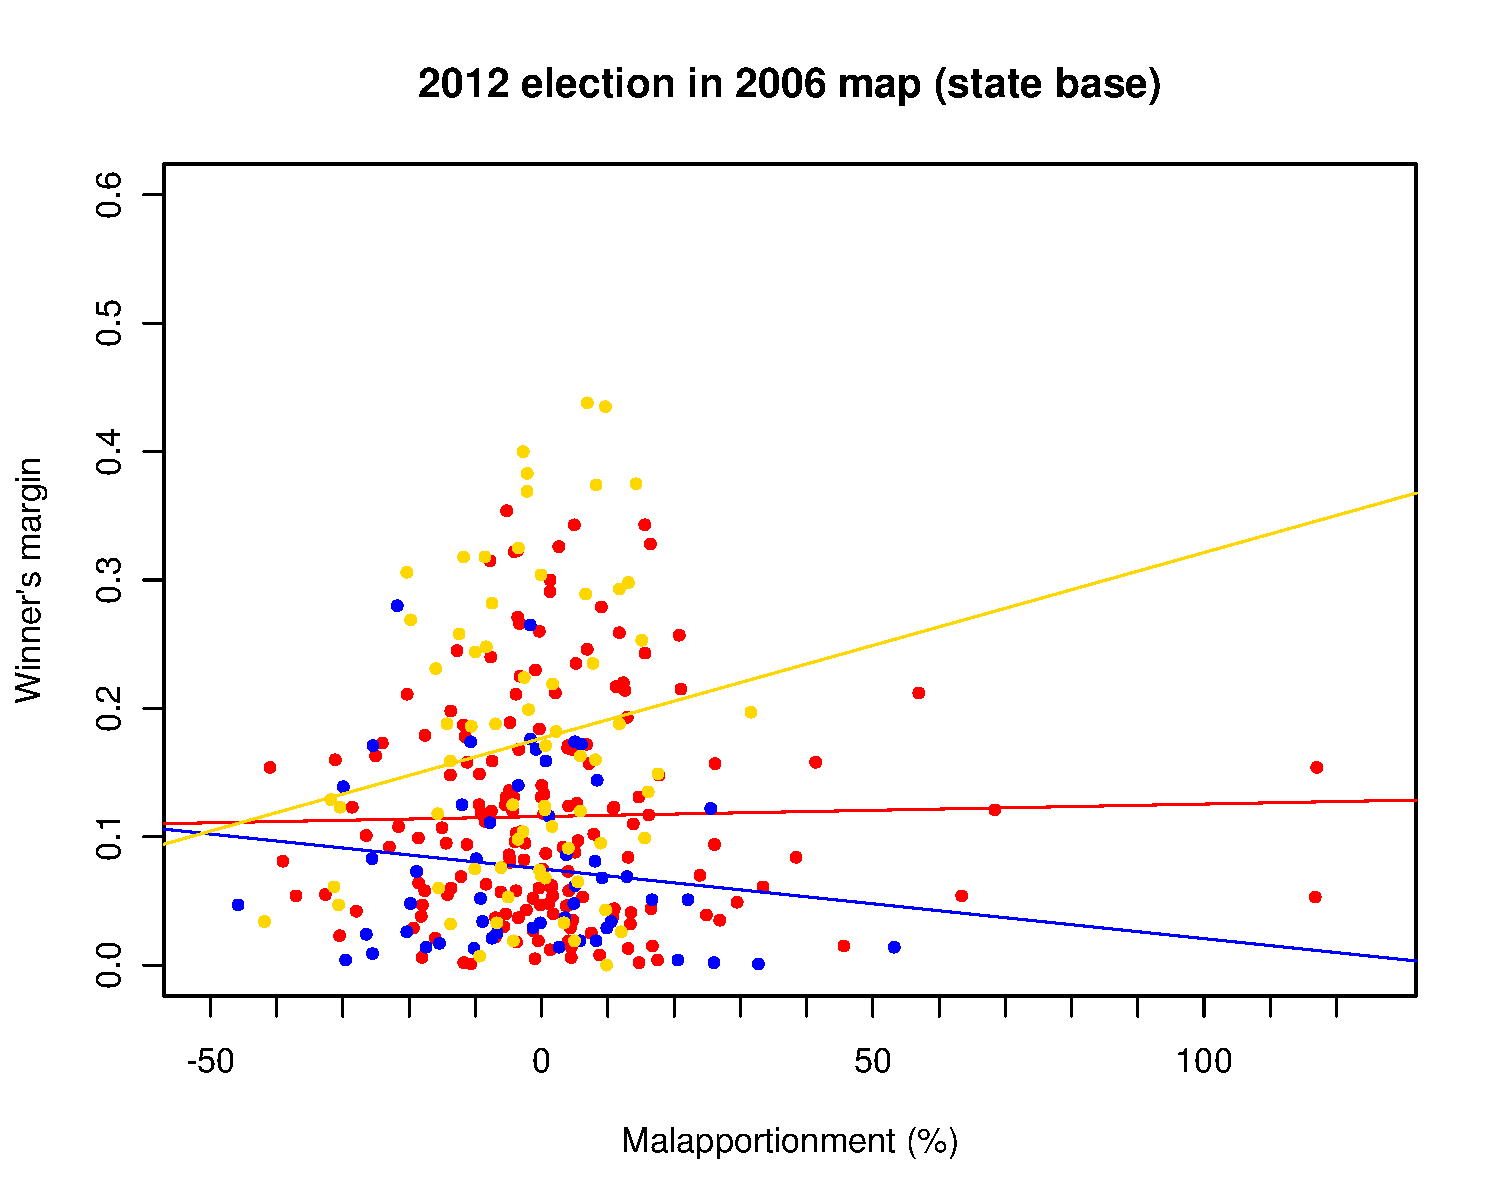
\includegraphics[width=.4\columnwidth]{malmg2012d0sta.pdf} & 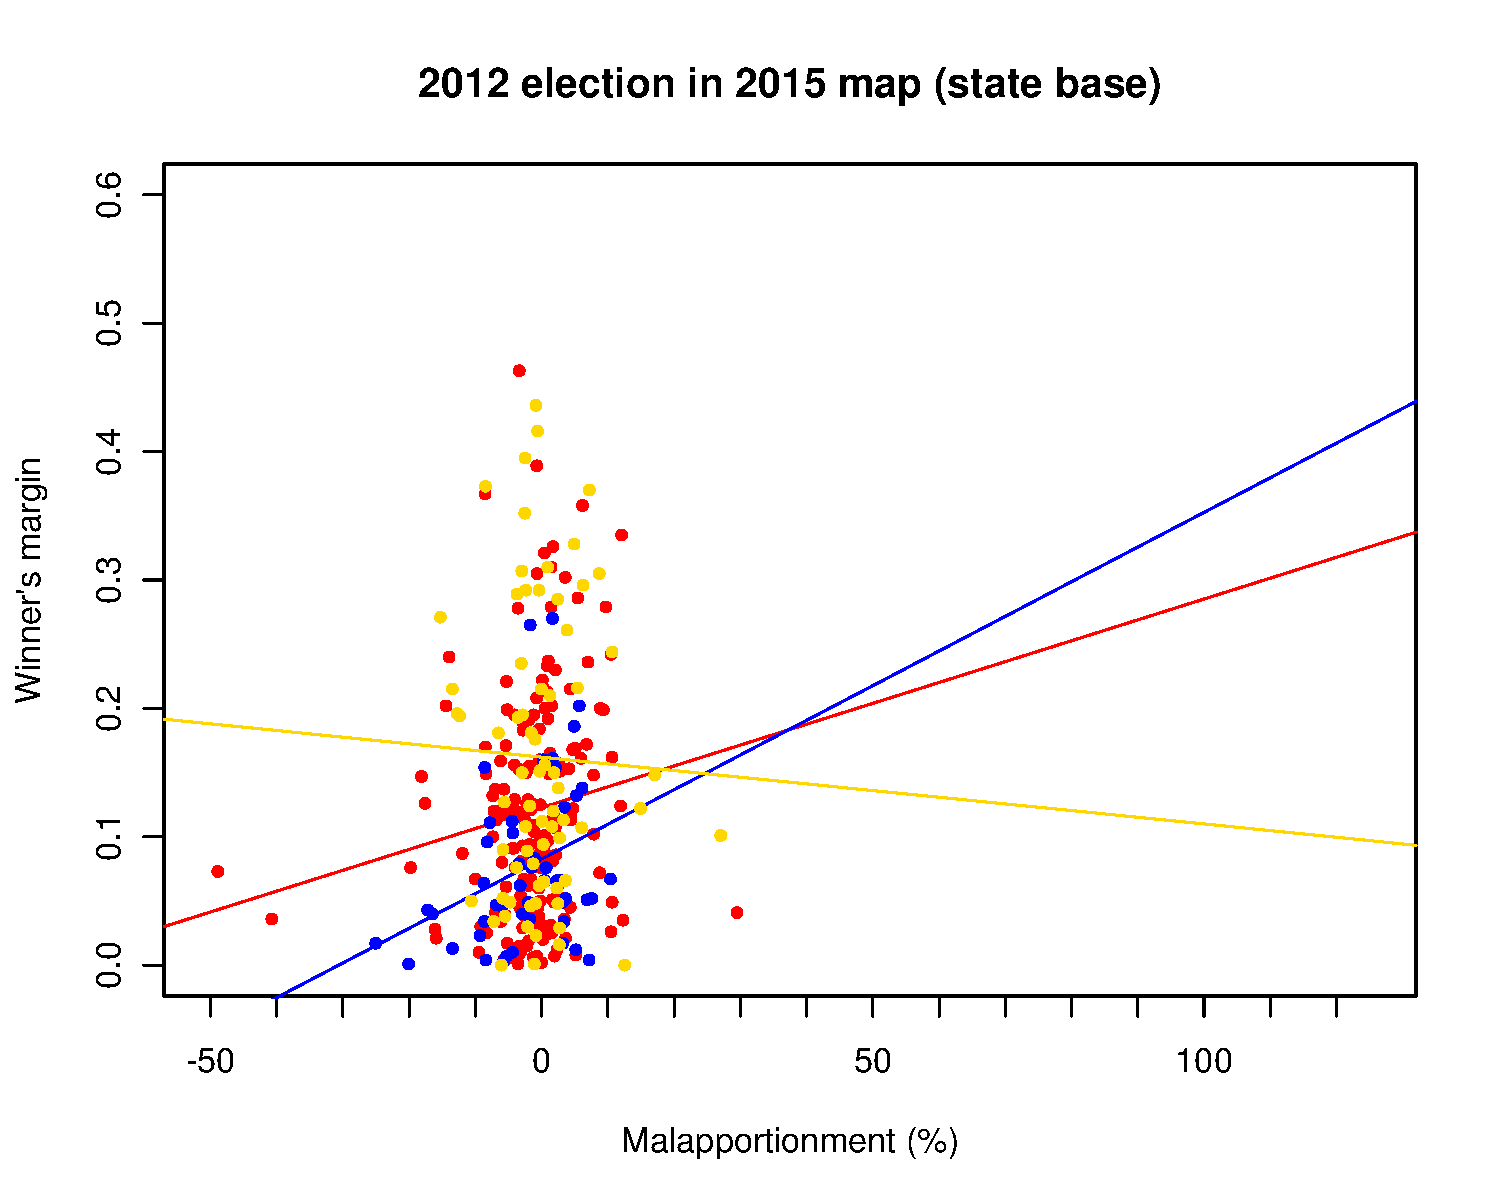
\includegraphics[width=.4\columnwidth]{malmg2012d3sta.pdf} \\
%   \end{tabular}
%   \caption{Vote margin and malapportionment (compared to state averages)}\label{F:malmgsta}
% \end{center}
% \end{figure}

% \begin{figure}
% \begin{center}
%   \begin{tabular}{cc}
%     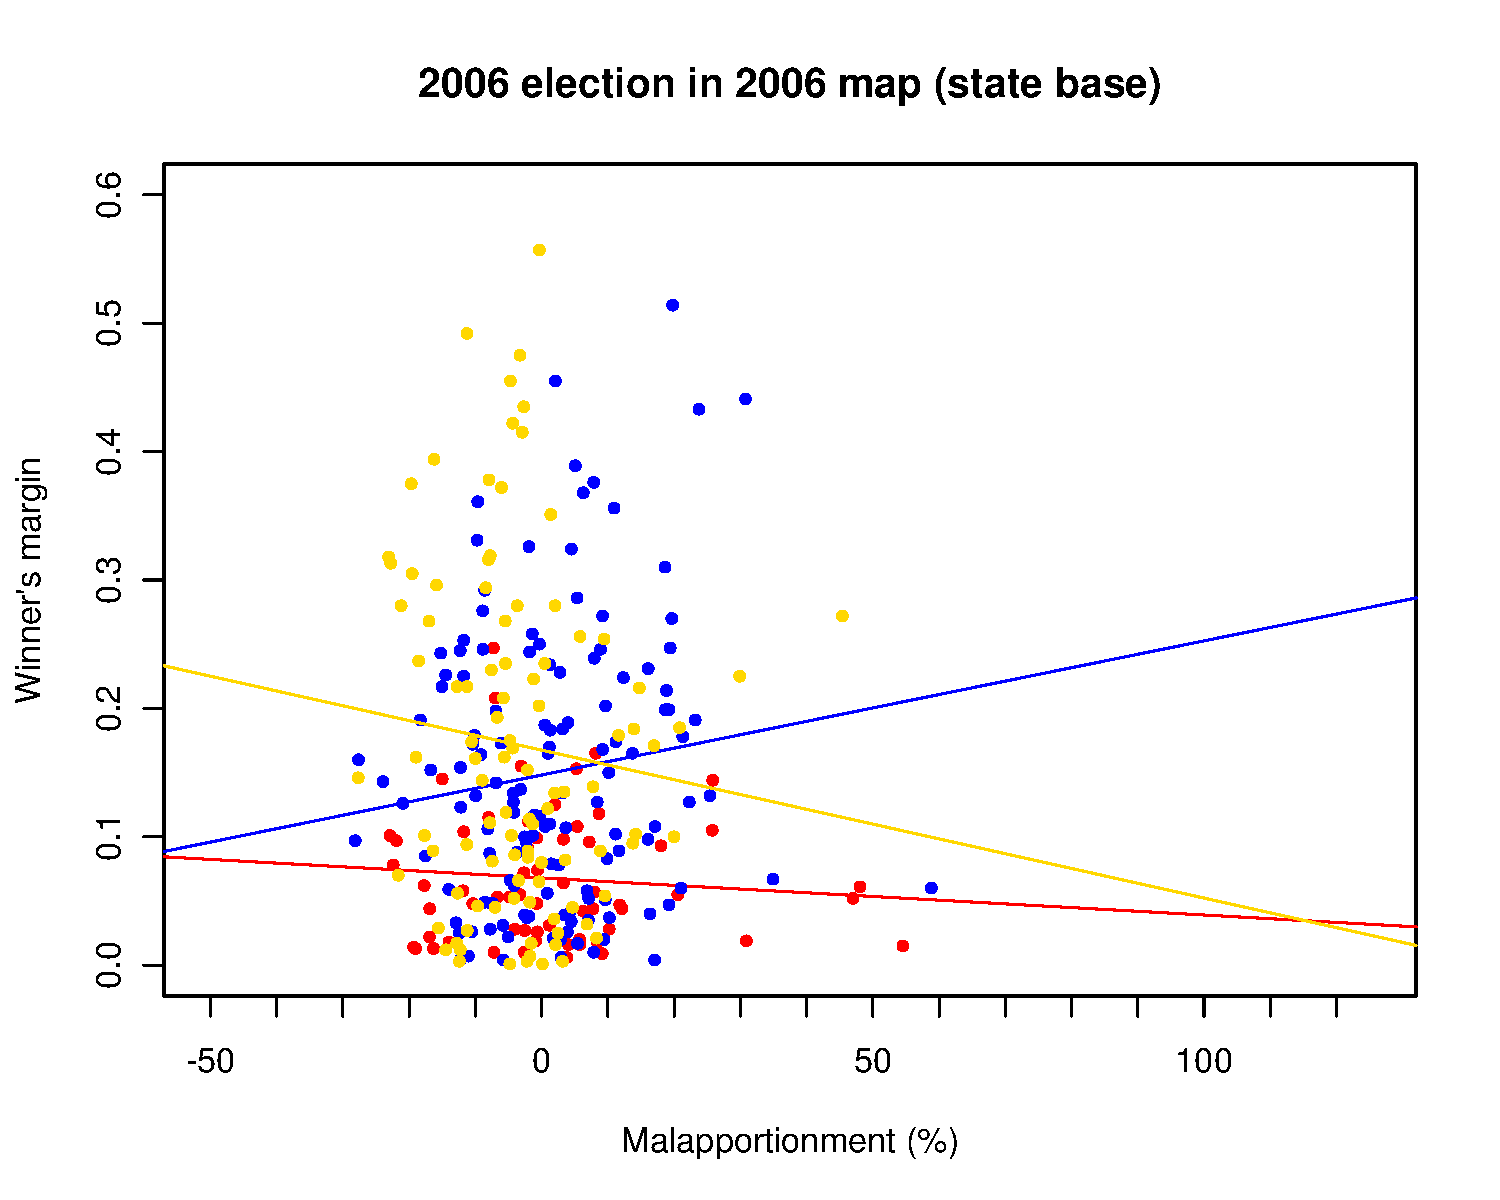
\includegraphics[width=.4\columnwidth]{malmg2006d0nat.pdf} & 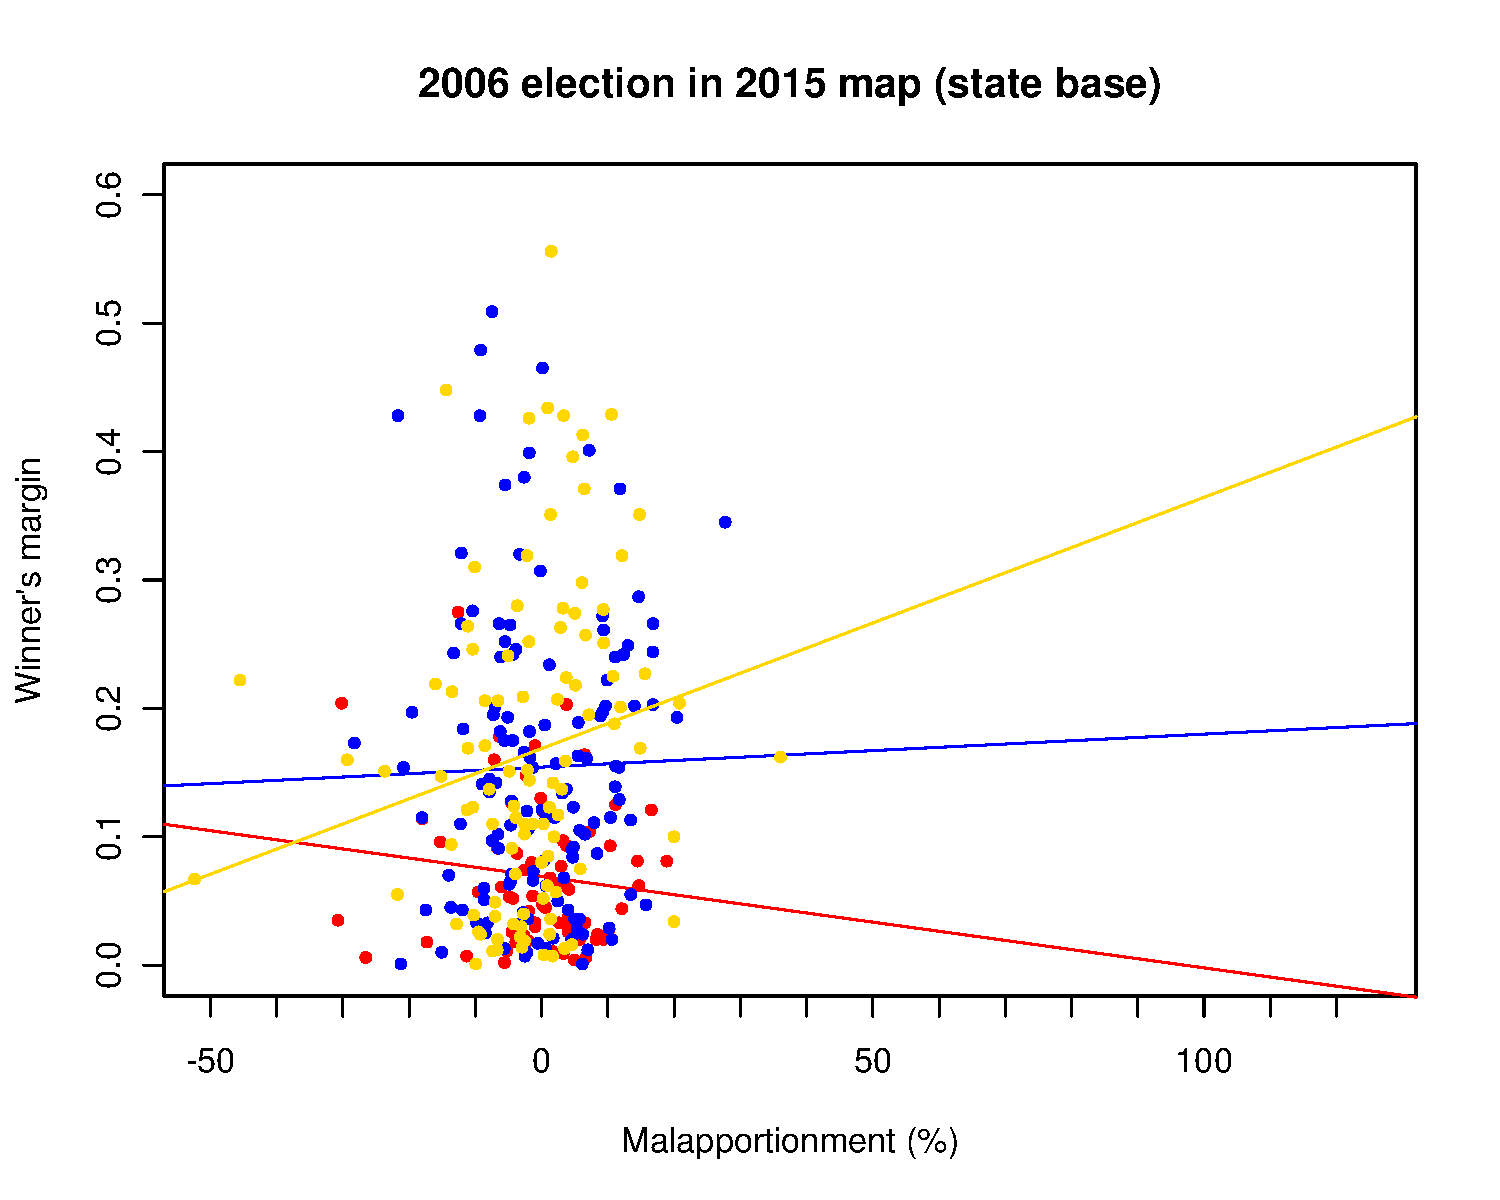
\includegraphics[width=.4\columnwidth]{malmg2006d3nat.pdf} \\
%     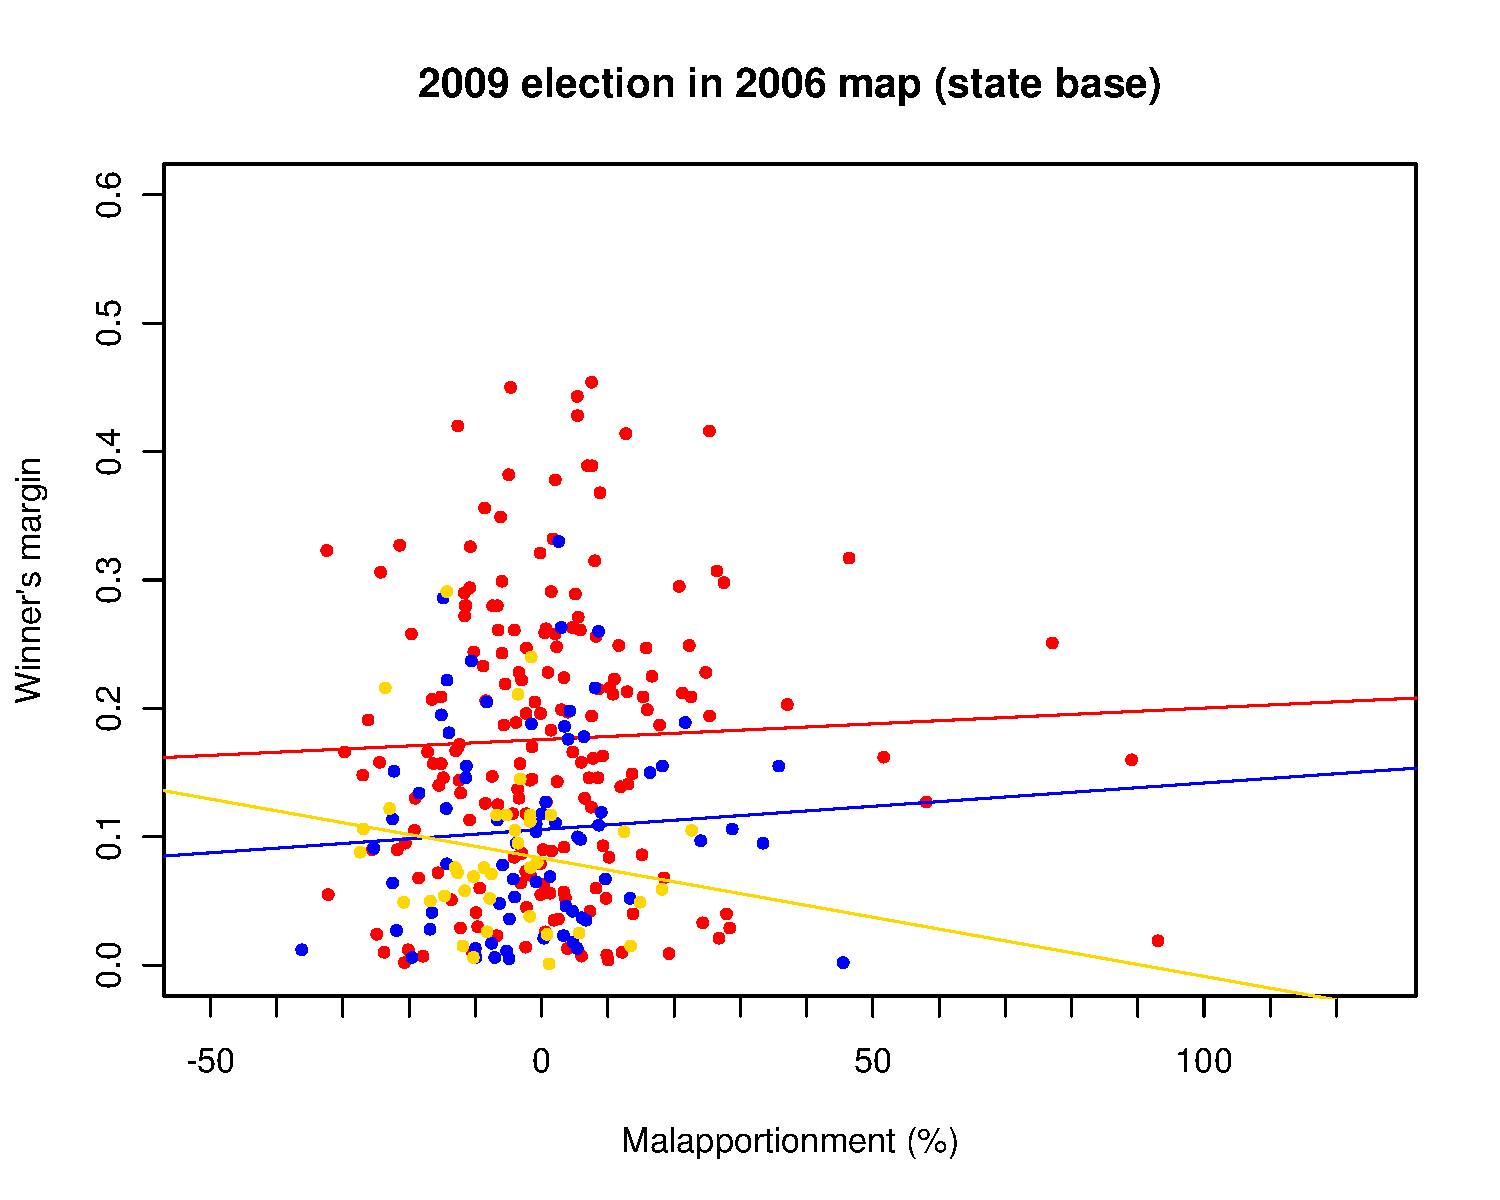
\includegraphics[width=.4\columnwidth]{malmg2009d0nat.pdf} & 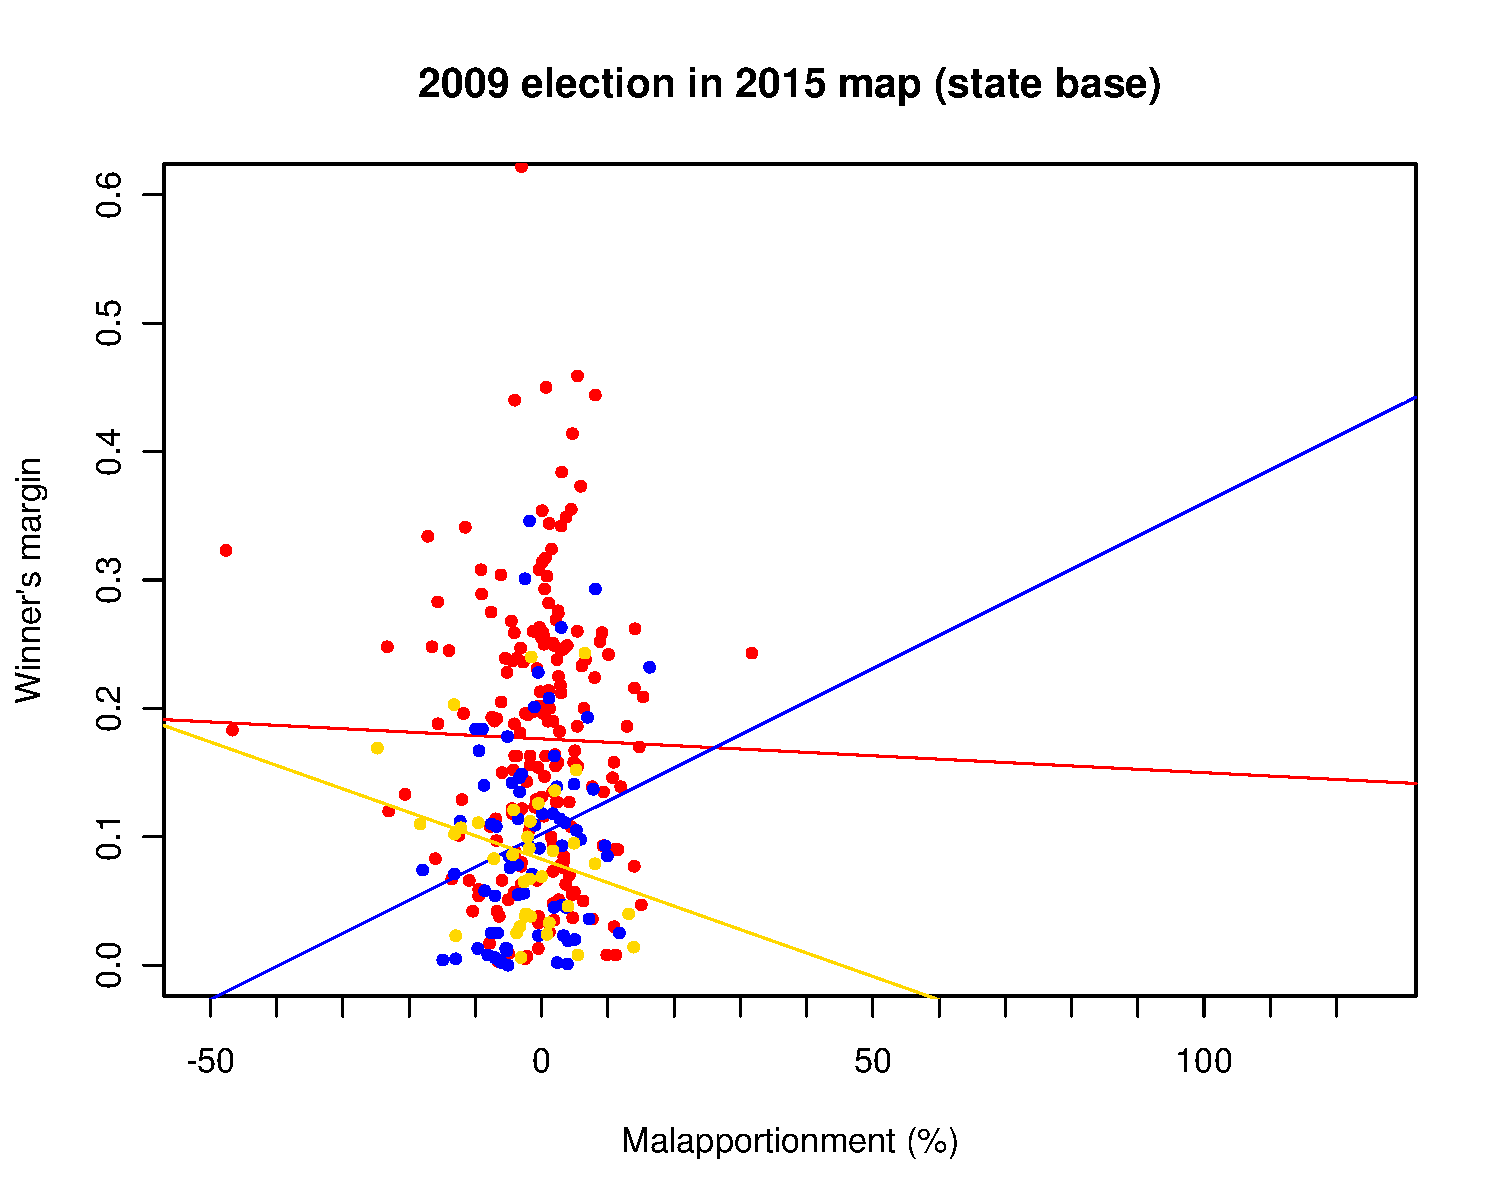
\includegraphics[width=.4\columnwidth]{malmg2009d3nat.pdf} \\
%     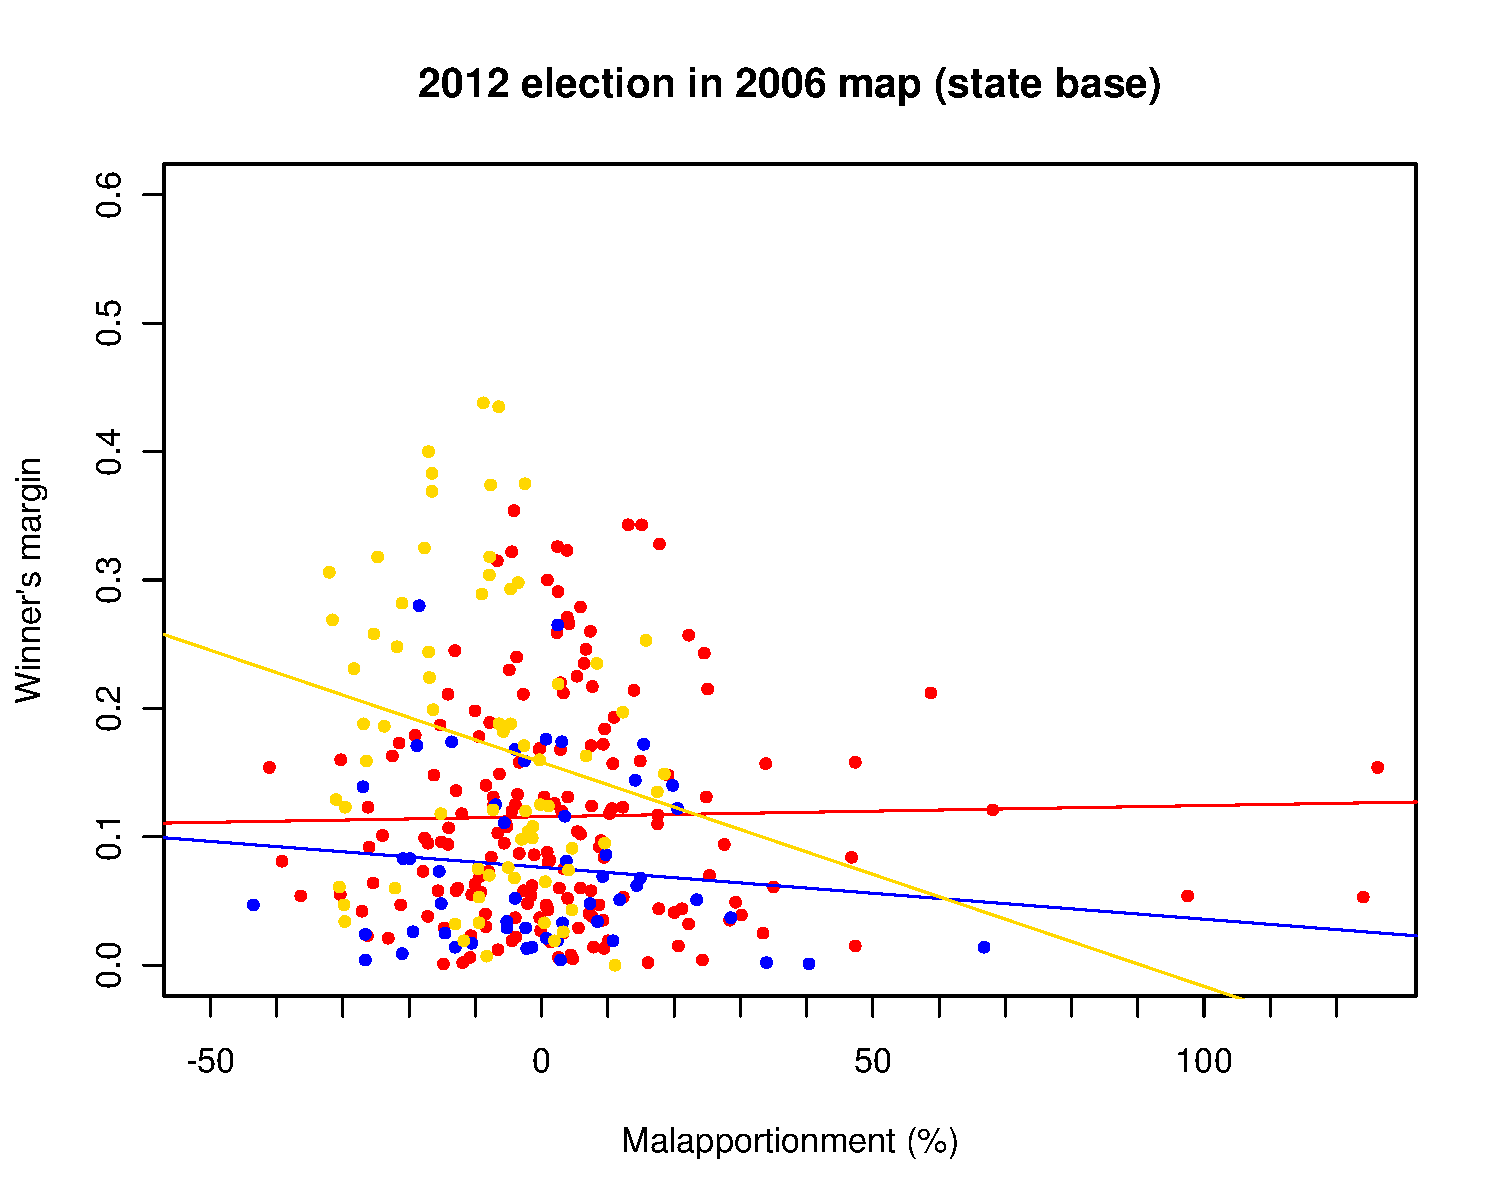
\includegraphics[width=.4\columnwidth]{malmg2012d0nat.pdf} & 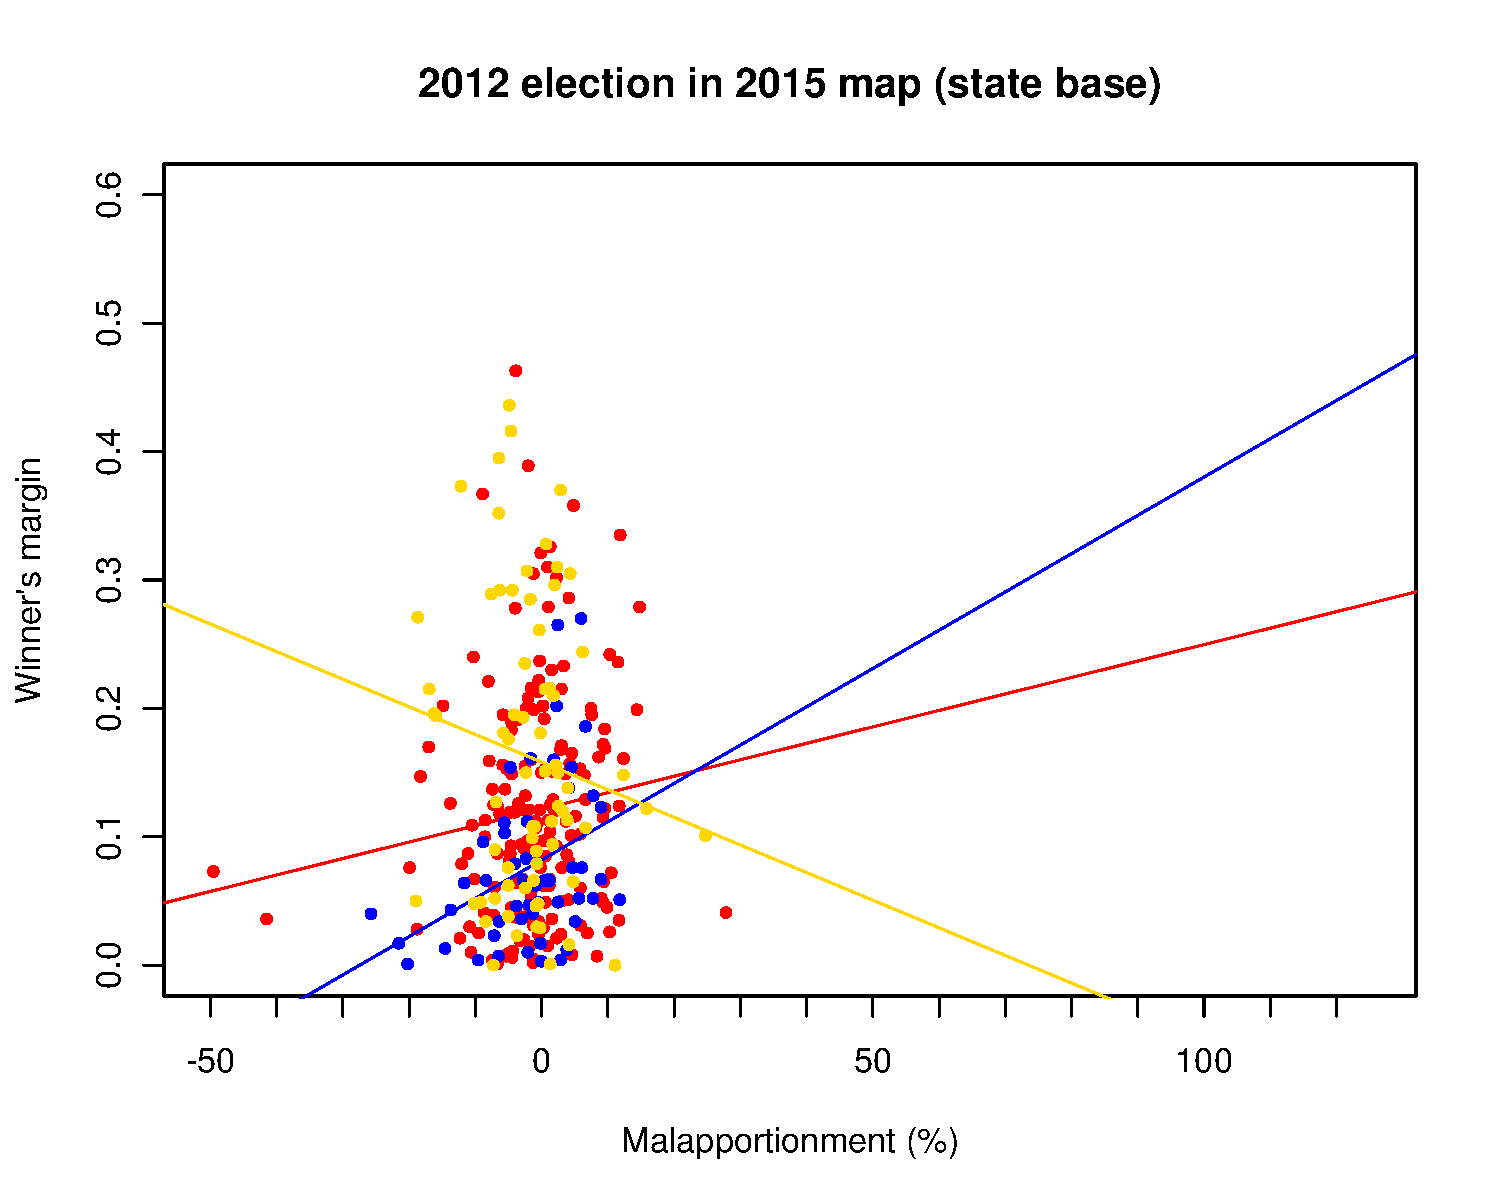
\includegraphics[width=.4\columnwidth]{malmg2012d3nat.pdf} \\
%   \end{tabular}
%   \caption{Vote margin and malapportionment (compared to national average)}\label{F:malmgnat}
% \end{center}
% \end{figure}

% Plots in Figures \ref{F:malmgsta} and \ref{F:malmgnat} 

\section{Seats--votes swing ratios}

This section offers a different, less common, but perhaps preferable approach to gauge differential effects of redistricting on the parties. It owes to \citet{niemi.fett1986swing}. The quantities of interest are \emph{seats--votes swing ratios} (or elasticities): the percentage change in seats associated with a one percent change in a party's national congressional vote. If the previous section aimed to measure this type of effect system-wide (the responsiveness parameter), swing ratios measure the sensitivity of individual parties’ seat shares to changes in voter preferences. A party with unity swing ratio can expect to receive its fair share of seats. Anything else indicates that parties can expect to win or lose more ($>1$) or less ($<1$) than one percent of seats for a unit percentage change in vote share. In pure PR systems, all parties' swing ratios should approximate one. Party swing ratio variance is expected in SMD systems, owing to margins, to the geography of votes, to turnout differentials, to malapportionment, to the number of competitors \citep{taagepera.shugart.1989}.

If swing ratios are straightforward conceptually, their estimation faces methodological challenges. Due to multifaceted changing circumstances from one election to the next, listed above, comparing two or more elections should be avoided \citep{jackmanMeasuringBias1994,niemi.fett1986swing}---removing the most obvious way of observing national vote shares vary. A counterfactual approach needs to be adopted, artificially giving party $X$ one percentage point above its actual vote. And this raises the question of tradeoffs: who loses when party $X$ wins? and where? In multi-party systems, the first question is not easy to answer a priori. All the pain can be felt by one party, by another, or by both in different proportions. When one party competes for the same voters as party $X$ does, it is even conceivable that both should increase their national vote together. The question of where is no less thorny. When a party with 10\% national support evenly spread across all districts earns one percent more, it should expect no change in seats won. When that same support is concentrated in one region, that difference nationwide will tip off the party in some districts, translating into more seats won.  

%When a party gains one percentage point in nationwide vote in a two party-system, the loss is attributable to the other party. Gauging seat share changes, however, will requires knowledge of district vote distributions---a 1\% change accross the board will tip only the most marginal of districts, but concentrating changes more heavily in some districts might tip those as well. Such challenges are more formidable in multiparty systems, where losses can be distributed differently across districts and opposition parties. 

\begin{figure}
\begin{center}
  \begin{tabular}{cc}
    (a) Three-way races & (b) Four-way races \\
    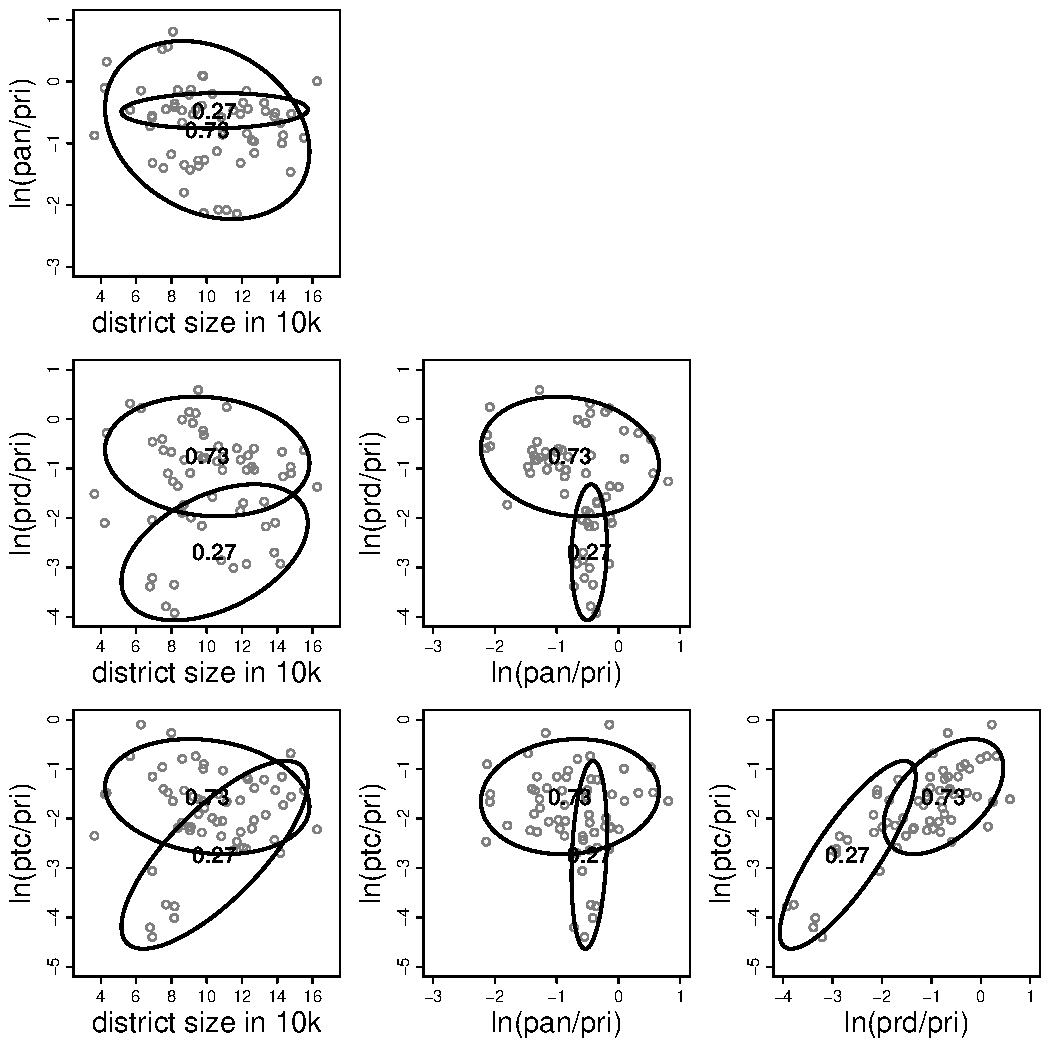
\includegraphics[width=.45\columnwidth]{linzerLogVot2009-1.pdf} &
    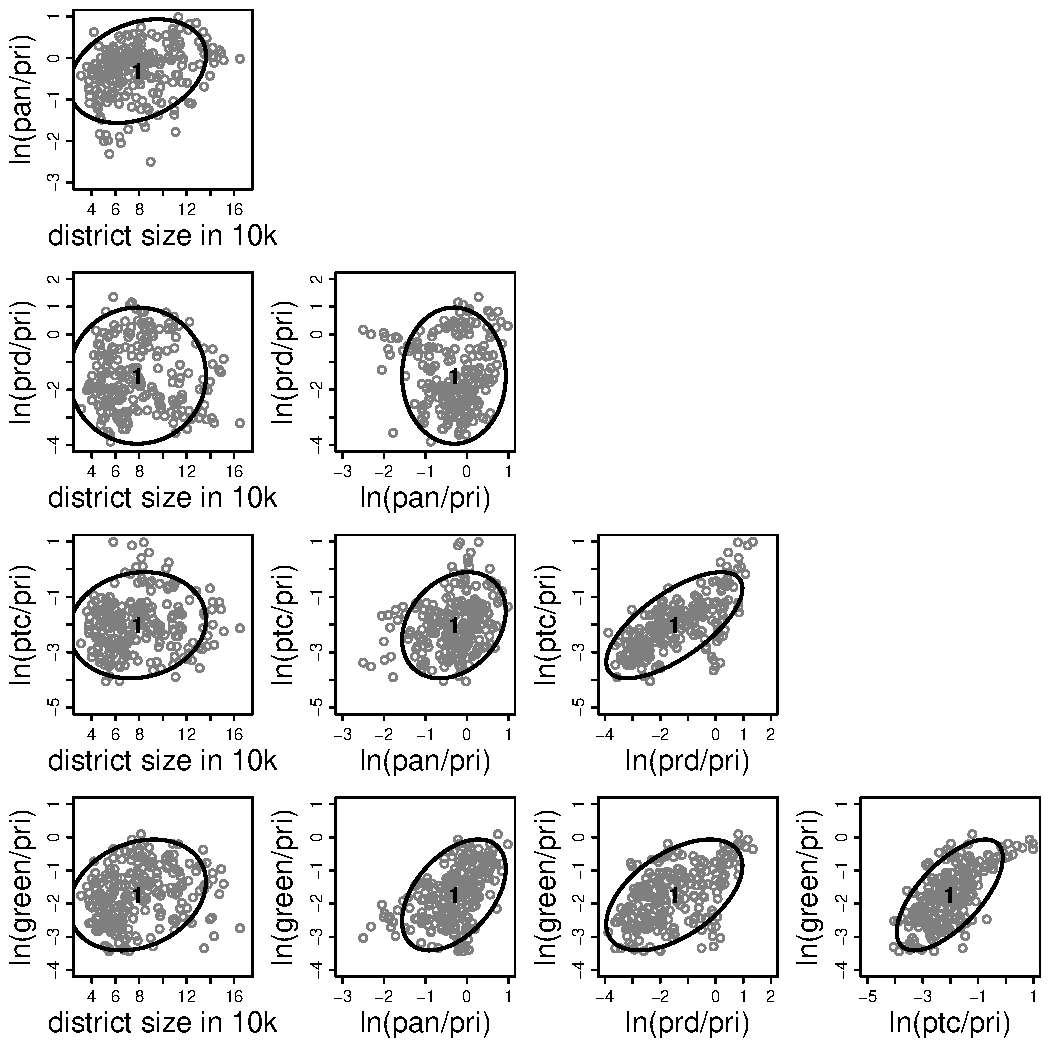
\includegraphics[width=.45\columnwidth]{linzerLogVot2009-2.pdf} 
  \end{tabular}
  \caption{Components and mix in the 2009 election. Panels report the log-ratio of party votes, using the PRI as reference to overcome the compositional nature of the data. Circles represent the multi-variate normal distributions that will be combined towards the estimated joint density. Numbers are the relative weights of the components.}\label{F:linzerLogVot}
\end{center}
\end{figure}

\citet{linzerSeatVoteElasticity2012} is a procedure overcoming both complictions with single-election district-level vote returns. The method relies on a finite mixture model for compositional data in order to estimate the joint probability density of parties' level of electoral support across districts. This joint distribution can inform, probabilistically, how changes in a party's vote share translate into losses, or perhaps gains, for the other parties at the district and the national levels, and thus deduce likely seat changes. The procedure extrapolates from the observed district party vote distributions, combining the properties of to or more multivariate normal into a composite density.\footnote{Mention how many components were used for the different contestations patterns in the code.} Figure \ref{F:linzerLogVot} shows (a) use of log-ratio vote shares (relative to PRI) to overcome compositional data bounds; (b) different patterns of pairwise party competition (ln(PRD/PRI) growth without affecting ln(PAN/PRI)). 

\begin{figure}
\begin{center}
    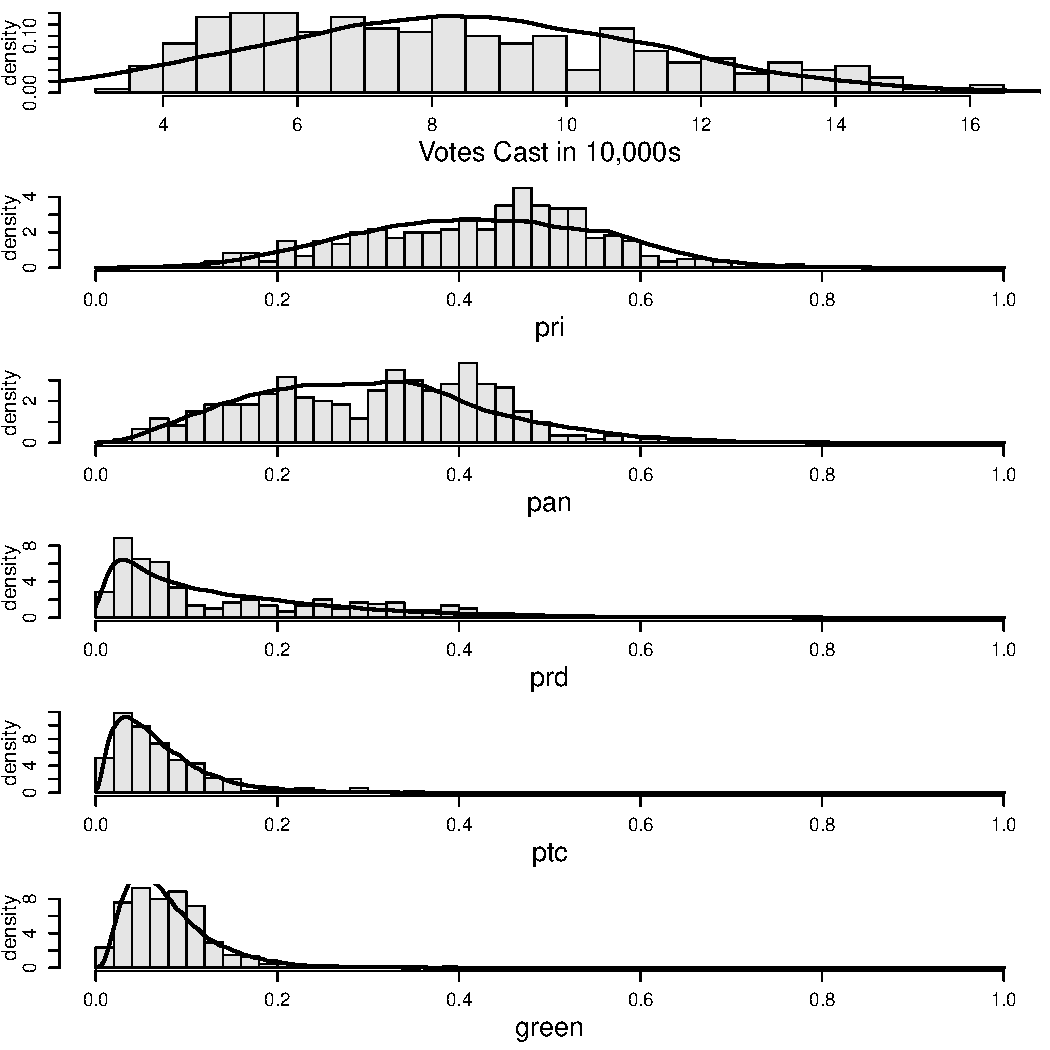
\includegraphics[width=.45\columnwidth]{linzerMarg2009.pdf}
  \caption{Fit of the finite mixture for 2009. Histograms report actual district party vote shares, lines are the marginals of the estimated 2009 election joint density.}\label{F:linzerMarginals}
\end{center}
\end{figure}

Figure \ref{F:linzerMarginals} to asses fit of estimated joint density. 

\begin{figure}
\begin{center}
  \begin{tabular}{cc}
    (a) Simulated vote shares & (b) Simulated seat shares \\
    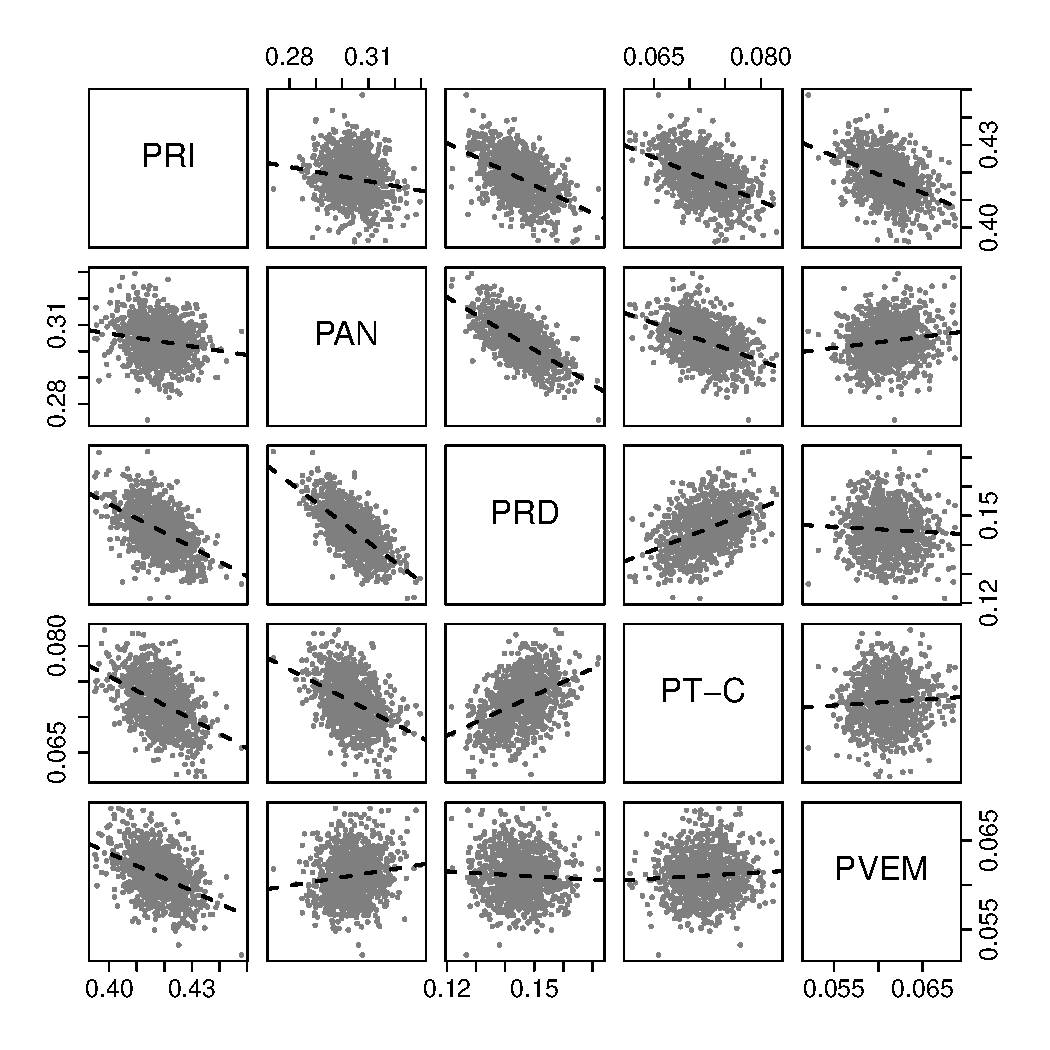
\includegraphics[width=.45\columnwidth]{linzerVoteSims2009.pdf} &
    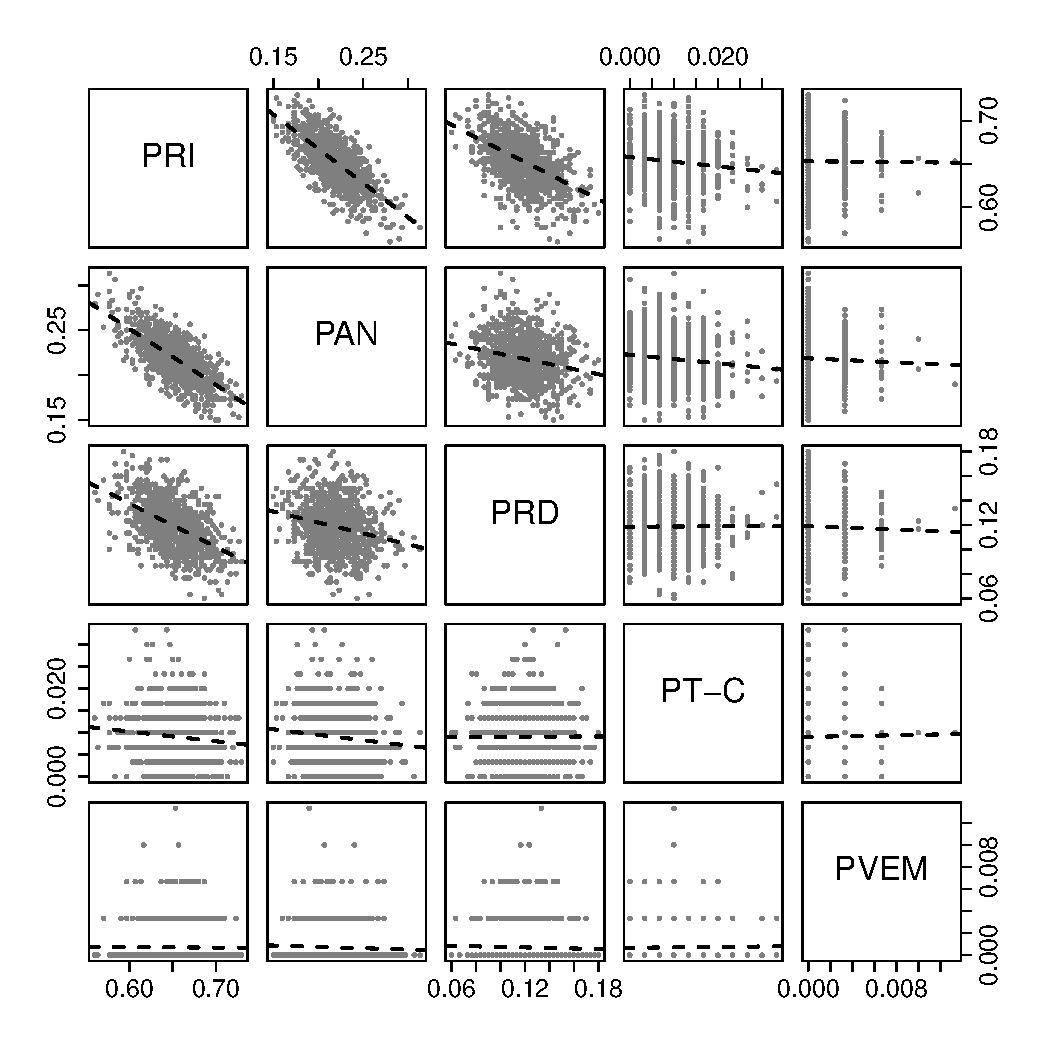
\includegraphics[width=.45\columnwidth]{linzerSeatSims2009.pdf} 
  \end{tabular}
  \caption{Covariance of party (a) vote shares and (b) seat shares in the 2009 election. Panels portray 1,000 elections simulated with the Linzer model, and the fit pf a linear regression.}\label{F:linzerSims}
\end{center}
\end{figure}

Monte-Carlo simulation to visit the vote and seat densities, and learn from them. Discuss the 1,000 simulated 2009 elections in Figure {F:linzerSims}. PRD growth votewise correlates with drops in the PRI vote and the PAN vote, but with increases in PT-C votes; PAN and PRD very negative in votes, but not in seats---their marginal districts are not against one another, but against the PRI. 

Seats--votes simulations for the 2006 and 2015 maps were generated for each election and party separately---single-election analysis offers the advantage of making temporal differences in party swing ratios available. Simulations were pooled, regressing simulates seats on simulated votes, a dummy indicating the 2015 map, and the simulated votes-dummy interaction. This approach has the advangage of offering a test of swing ratio differences attributable to the change in maps. 

$S_{p,m} = \beta_0 + \beta_1 V_{p,m} + \beta_2 dMap2015_m + \beta_3 V_{p,m} \times dMap2015_m + \texttt{error}_{p,m}$


\begin{table}
\centering
\begin{tabular}{lrrrrrr}
                   & \multicolumn{2}{c}{PAN}   & \multicolumn{2}{c}{PRI}   & \multicolumn{2}{c}{Left}   \\
                   & $\hat{\beta}$ & $p$ & $\hat{\beta}$ & $p$ & $\hat{\beta}$ & $p$  \\ \hline
~~\textbf{2006 election} \\
$V$                &     1.94 & $<.001$&   2.27 &$<.001$&   1.91 &$<.001$\\
$V \times$ dis2015 &     +.45 & $<.001$&  $-.01$&  .809 &  $-.04$&  .183 \\
~~\textbf{2009 election} \\
$V$                &     1.95 & $<.001$&   2.27 &$<.001$&   1.67 &$<.001$\\
$V \times$ dis2015 &    $-.13$&   .003 &   +.04 &  .354 &  $-.02$&  .623 \\
~~\textbf{2012 election} \\
$V$                &     2.24 &$<.001$ &   3.99 &$<.001$&   2.39 &$<.001$\\
$V \times$ dis2015 &     +.02 &   .604 &   +.03 &  .720 &  $-.06$&  .103 \\ \hline
\end{tabular}
\caption{Comparative 2006 and 2015 map seats--votes swing ratios. $\hat{\beta}$ are estimated coefficients of party seat shares regressed on vote shares ($V$) and vote shares-redistricting interaction ($V \times$ dis2015) and the corresponding $p$-values, using data simulated with the \citet{linzerSeatVoteElasticity2012} finite mixture method. A constant and a redistricting dummy were also included in the right side but are not reported. See text for details.} 
\end{table}

\section{Electoral volatility}

* * To be written * * May help explain why malapportionment has no larger consequences. 

One factor that may explain the absence of party bias is electoral volatility. By being larger than malapportionment, it may be ecplipsing its potential to create bias...

Noting that victory margins began widening in the mid-1960s, \citet{mayhew1974vanishingMg} saw gerrymandering as one possible explanation, incumbents influencing the preservation of safe districts. While the argument opened the heated incumbency advantage debate, the intuition may guide our inquiry. District volatility should capture a key element for analysis of map similarities. District $d$ volatility is $v_d = 1/2 \sqrt{ \sum_{p=1}^P \sum_{t=2}^3 (v_{d,p,t}- v_{d,p,t-1})^2 }$ with $p$ indexing the competing parties and $t=1,2,3$ for the 2006,  2009, and 2012 congressional elections respectively.\footnote{The measure of volatility proposed is inspired in measures of disproportionality, replacing the seats--votes difference with vote first differences. It is a squared version of a Loosemore-Hanby index \citep{loosemore.hanbyDisproportionality1971,gallagherDisproportionality1991}.} 

Mexican party strength is not proportional to the formidable entry barriers they enjoy and massive public subsidies they receive yearly \citep{magar.2007ref.2015}. Evidence of this is their inability to cultivate loyal voters. District volatility is remarkably high, as shown in Table \ref{T:volatMarginsd0}. The median district saw 25 percent of votes change party hands between 2006 and 2012 (not exactly how the index reads, but close enough). With so many volatile districts around, parties should have attempted to redress strongholds that automated redistricting split beyond recognition. How much were strongholds affected by the initial 2015 proposal? To what extent did party counter-proposals redress them? This should be a promising line of inquiry. 

\begin{table}
\begin{center}
\begin{tabular}{lrrrrr}
                    &  min.   &  25\%   & median  & 75\%   & max \\ \hline
district volatility &  .08    & .19     & .25     & .31    & .52 \\
mean PAN margin     &  $-.49$ & $-.23$  & $-.10$  & .01    & .28 \\   
mean PRI margin     &  $-.43$ & $-.09$  & $-.01$  & .07    & .28 \\   
mean PRD margin     &  $-.51$ & $-.31$  & $-.21$  & $-.04$ & .39 \\
\end{tabular}
\caption{2006 map district volatility and party margins in three congressional elections}\label{T:volatMarginsd0}
\end{center}
\end{table}

% comment [Eric] One possibility is regressing new district similarity on mean 2006--12 parent district margin, low volatility, and their interaction. Another route is the estimation of district elasticities---how vote swings in a district's \emph{secci\'ones} respond to statetwide party swings. This could provide an alternative approach to explain the district similarity index. The appendix has preliminary elasticity estimates and some discussion.


\section{Conclusion}

** To be written **

Mexico's federal districts exhibit no party bias when analyzed at the state level. Big system responsiveness, typical of first-past-the-post system in units with few federal districts, is associated with the districts. So PRI's tendency to be over-represented more than PAN and PRD, and the PRI's winning of a couple extra seats with the redistricting proposal is not the product of partisan bias. If the PRI wins more this is due to its status as the largest party in more states that the other two major parties combined. 

\section*{Appendix 1: code}

\begin{footnotesize}
\begin{verbatim}
bugsModel <- function() {
    for (i in 1:I){     # loop over state-years
        for (j in 1:J){ # loop over parties (dummy selects those who ran that year) 
            S[i,j] ~ dbin(pi[i,j], D[i])  # D is number SMD seats in obs. i's state
        }
        numerator[i,1] <- dummy[i,1] * exp( lambda[1] + rho * log(v[i,1]) )
        numerator[i,2] <- dummy[i,2] * exp(             rho * log(v[i,2]) )
        for (j in 3:J){
            numerator[i,j] <- dummy[i,j] * exp( lambda[j-1] ) * v[i,j]^rho
        }
        for (j in 1:J){ # loop over parties (dummy selects those who ran that year) 
            d1[i,j] <- dummy[i,1] * exp( lambda[1] ) * v[i,1]^rho 
            d2[i,j] <- dummy[i,2]                    * v[i,2]^rho 
            d3[i,j] <- dummy[i,3] * exp( lambda[2] ) * v[i,3]^rho 
            d4[i,j] <- dummy[i,4] * exp( lambda[3] ) * v[i,4]^rho 
            d5[i,j] <- dummy[i,5] * exp( lambda[4] ) * v[i,5]^rho 
            d6[i,j] <- dummy[i,6] * exp( lambda[5] ) * v[i,6]^rho 
            d7[i,j] <- dummy[i,7] * exp( lambda[6] ) * v[i,7]^rho 
            denominator[i,j] <- d1[i,j]+d2[i,j]+d3[i,j]+d4[i,j]+d5[i,j]+d6[i,j]+d7[i,j]
            pi[i,j] <- numerator[i,j] / denominator[i,j]
        }
    }
    ### priors
    for (p in 1:6){ # there are 7 party labels in the 3-election data, PRI is reference
        lambda[p] ~ dnorm( 0, tau.lambda )
    }
    tau.lambda <- pow(.25, -2)
    rho ~ dexp(.75) # this has positive range, median close to 1, mean 1.25, max 4.5
}
\end{verbatim}
\end{footnotesize}

\section*{Appendix 2: elasticity} 

% Adding more election cycles will improve the estimates. Two points now for each line as of now. 

Different from \citet{linzerSeatVoteElasticity2012}. An approach of this kind may be useful for the party interactions paper: which secciones are more valuable for a party, and how do parties respond to the algorithm regarding these secciones?

How elastic a district is to a party's statewide (nationwide?) vote swings is interesting. Elasticity should shape redistricting preferences. A district is highly elastic for the PAN when small shifts in the party's vote statewide correspond to sharp district vote hikes. It is inelastic when it corresponds to more modest district vote changes. Negative elasticity is even conceivable, the district vote growing when the rest of the state shrinks. Local effects on mobilization and voting can move against state effects. If every \emph{secci\'on} in the district is a microcosm of the state's electorate, unit elasticity ensues. 

The measure regresses a party's three-year vote change in the \emph{secci\'on} $\Delta_s$ on the the parent state vote change $\Delta_e$ thus:  

\begin{equation}
\Delta_s = \sum\limits_{d=1}^{D_e} \alpha_d + \beta_d \Delta_e.
\end{equation}

\noindent Fixed effects for each district are considered, fitting separate $\alpha_d$ and $\beta_d$ regression coefficients for every district (indexed $d$). The model is estimated for every state separately because doing it nationwide involves too many \emph{secciones} (67k) and parameters (600) for my machine. 

\begin{figure}
\begin{center}
  \begin{tabular}{cc}
    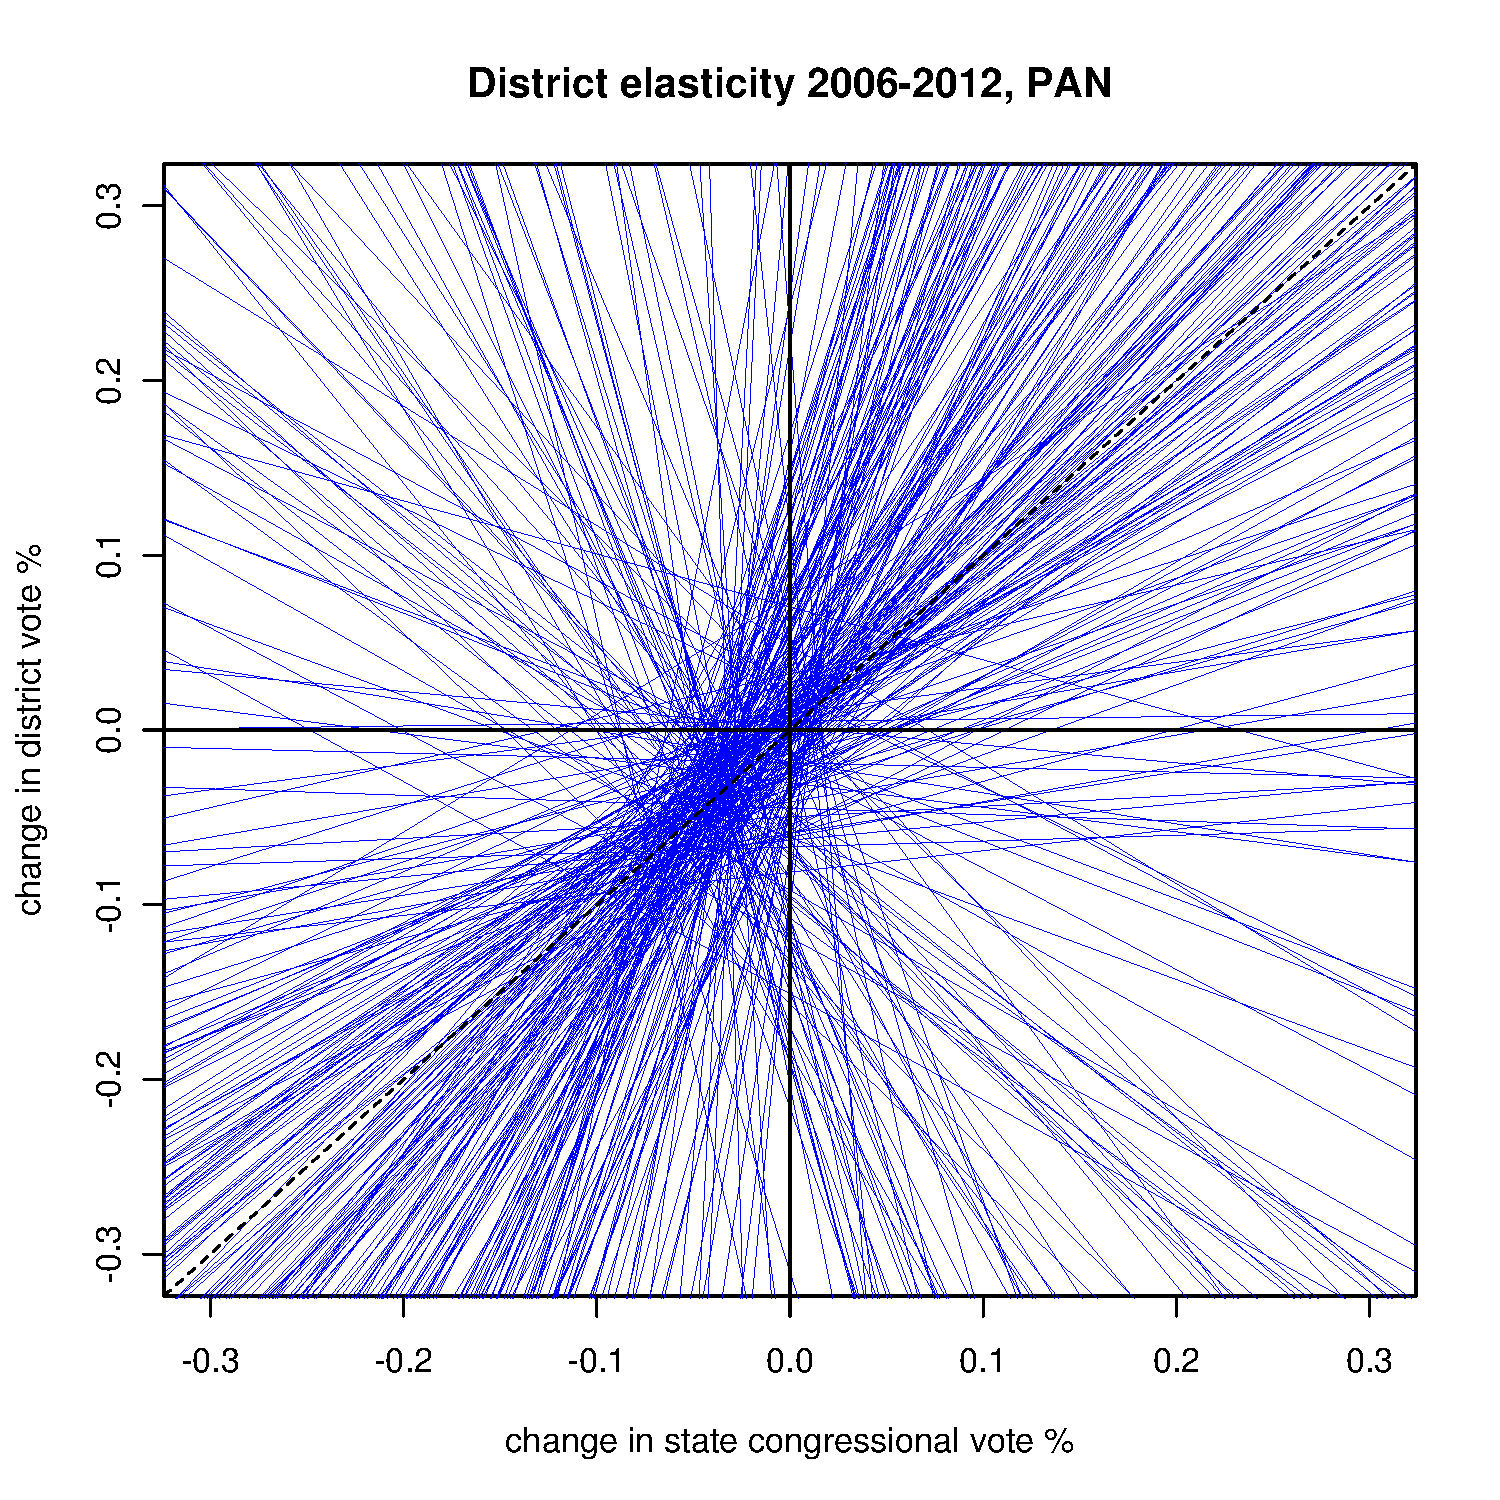
\includegraphics[width=.4\columnwidth]{elastpand0.pdf} & 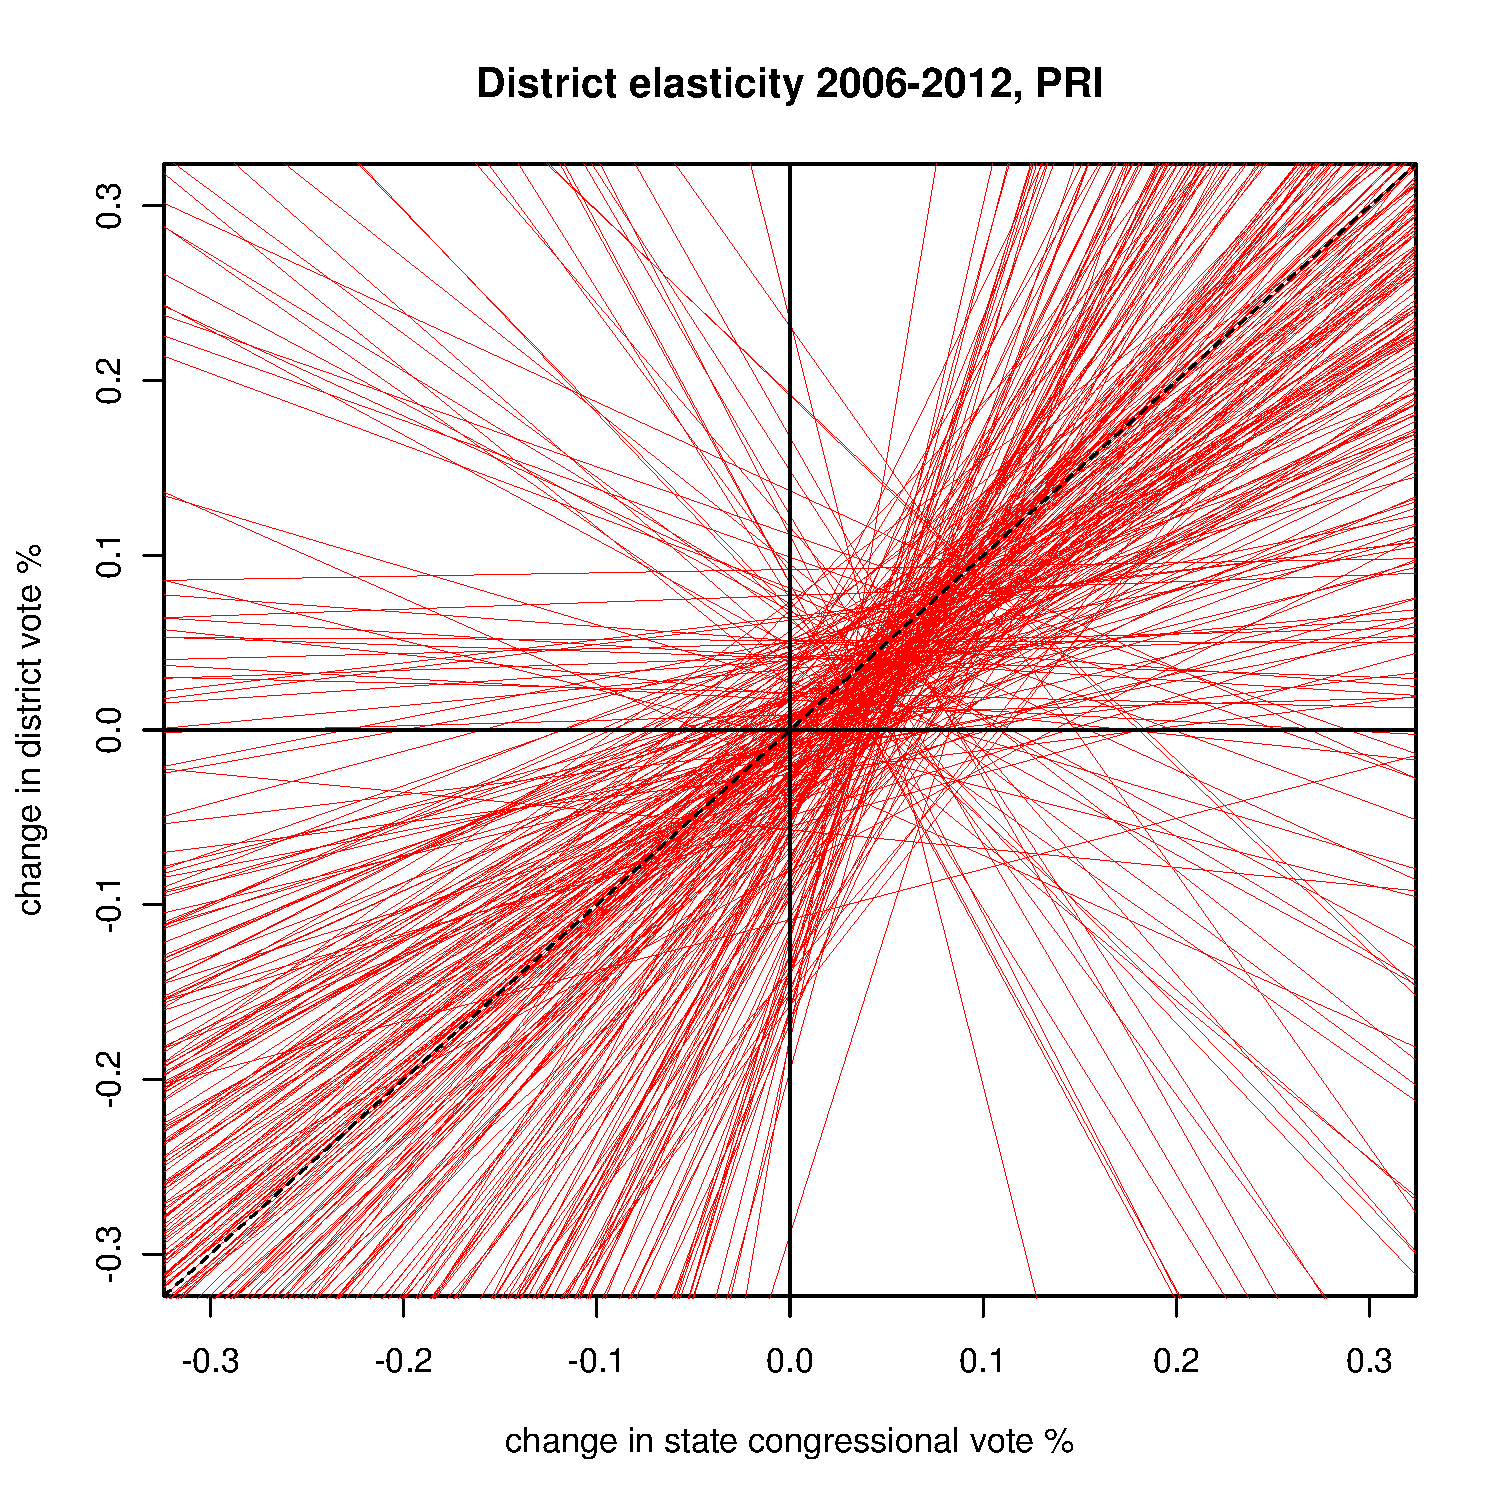
\includegraphics[width=.4\columnwidth]{elastprid0.pdf} \\
    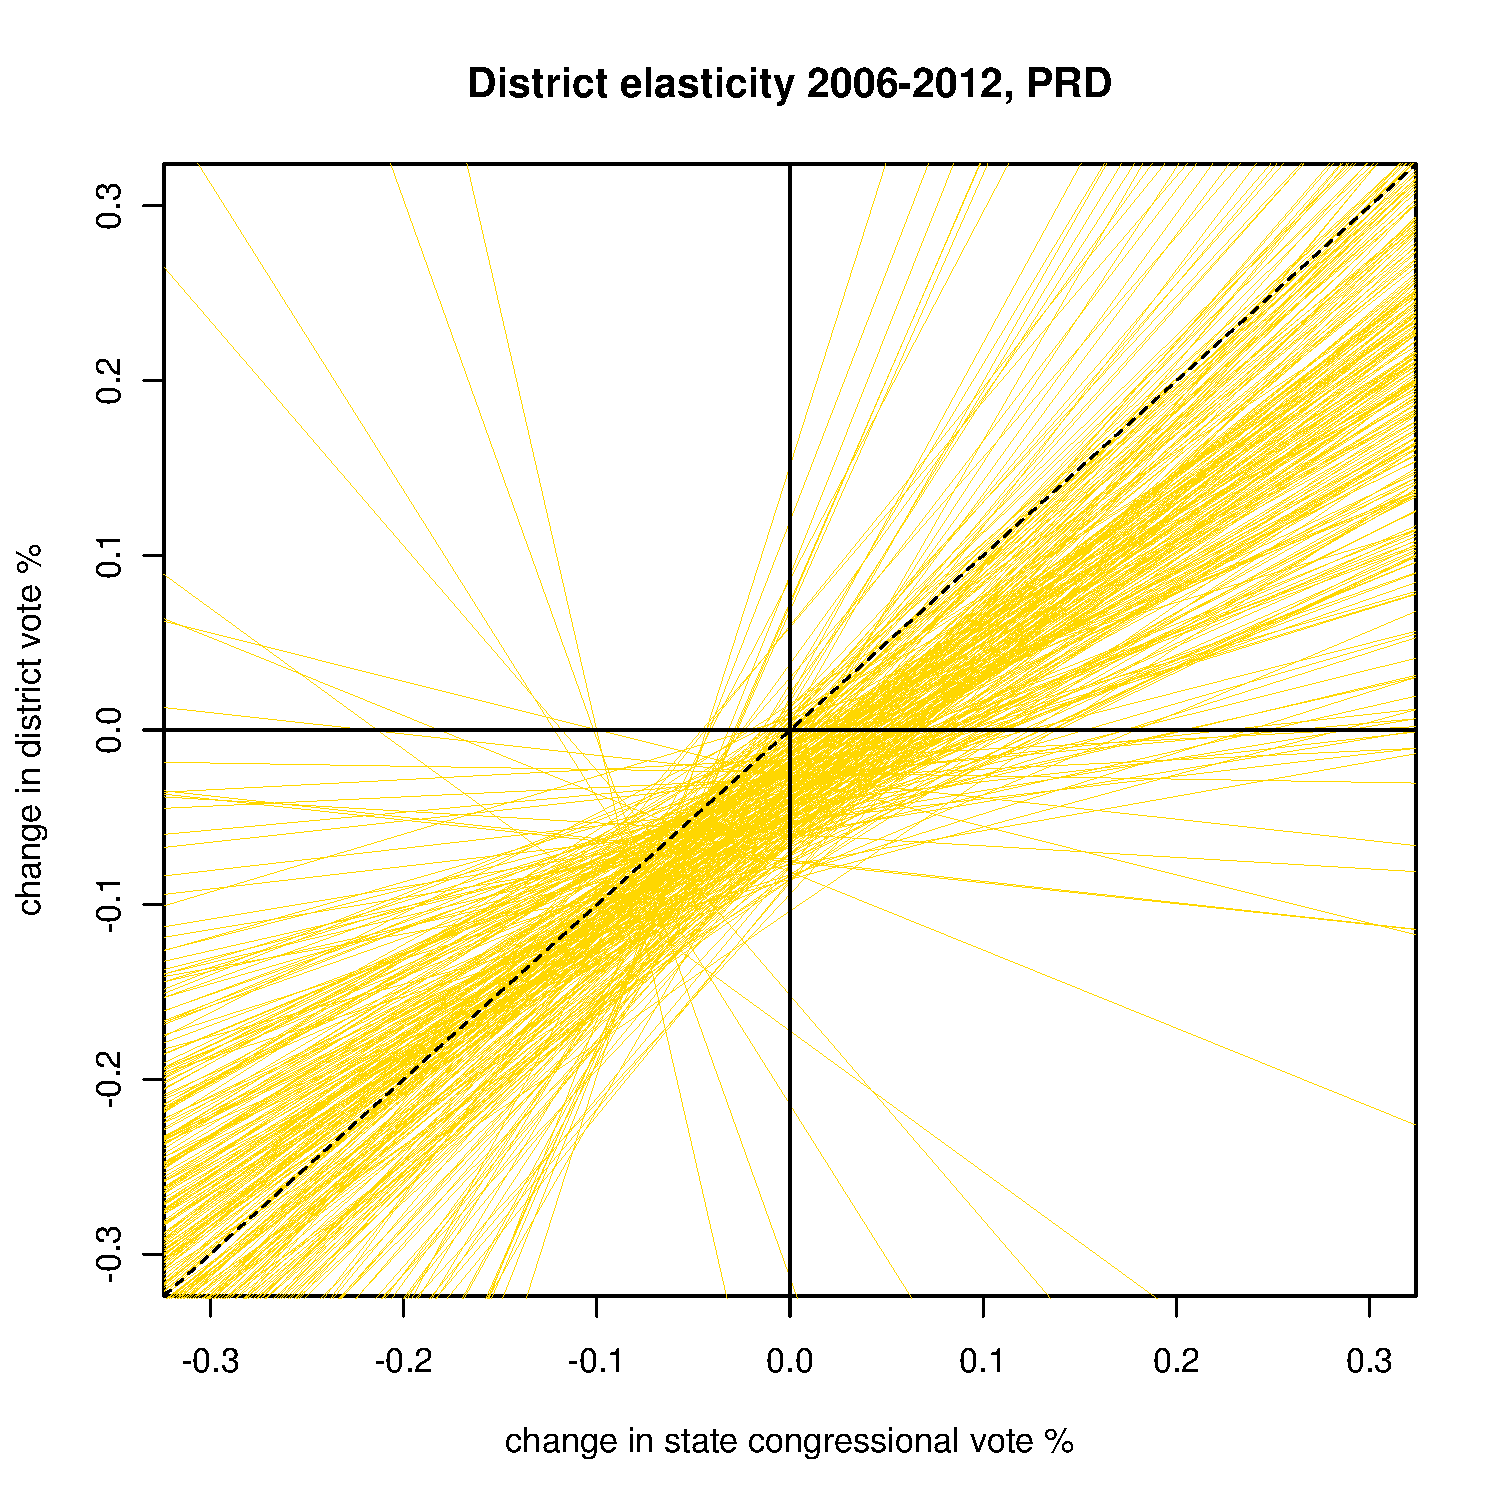
\includegraphics[width=.4\columnwidth]{elastprdd0.pdf} &  \\
  \end{tabular}
  \caption{Parties' district elasticities}\label{F:malmgnat}
\end{center}
\end{figure}


\bibliographystyle{apsr}
%\bibliography{../bib/redMex}
\bibliography{../bib/magar}

%% next command, in console, extracts only relevant paper references to extracted.bib (http://tex.stackexchange.com/questions/41821)
%bibexport -o extracted.bib myarticle.aux

\end{document}
